\documentclass[]{beamer}
% Class options include: notes, notesonly, handout, trans,
%                        hidesubsections, shadesubsections,
%                        inrow, blue, red, grey, brown

% Theme for beamer presentation.
\usepackage{beamerthemesplit} 



% Other themes include: beamerthemebars, beamerthemelined, 
%                       beamerthemetree, beamerthemetreebars  

\title{PHY250}    % Enter your title between curly braces
\author{Anabela R. Turlione}                 % Enter your name between curly braces
\institute{Digipen}      % Enter your institute name between curly braces
\date{Fall 2021}                    % Enter the date or \today between curly braces


\begin{document}

% Creates title page of slide show using above information
\begin{frame}
  \titlepage
\end{frame}
%\note{Talk for 30 minutes} % Add notes to yourself that will be displayed when
                           % typeset with the notes or notesonly class options

\section[]{}

% Creates table of contents slide incorporating
% all \section and \subsection commands
\begin{frame}
  \tableofcontents
\end{frame}

%%%%%%%%%%%%%%%%%%%%%%%%%%%%%%%%%%%%%%%%%%%%%%%%%%%%%%%%%%%%%%%%%%%
\section{Electromagnetic waves}
\subsection{Introduction}

%%%%%%%%%%%%%%%%%%%%%%%%%%%%%%%%%%%%%%%%%%%%%%%%%%%%%%%%%%%%%%%%%%%
\begin{frame}
\frametitle{Introduction}


\begin{itemize}
 \item  Changing Magnetic Field $\rightarrow$ Changing Electric Field
\pause 

\item Changing Electric Field $\rightarrow$ Changing Magnetic Field
\end{itemize}

\vspace{3mm}


\textbf{Electromagnetic Wave}: Wave of Electric and Magnetic Field
\pause
\vspace{3mm}

Changing Electric Field $\rightarrow$ Changing Magnetic Field$\rightarrow$ Changing Electric Field 

\pause
\vspace{3mm}

The light is an electromagnetic wave that can propagate through space.

  \end{frame}

%%%%%%%%%%%%%%%%%%%%%%%%%%%%%%%%%%%%%%%%%%%%%%%%%%%%%%%%%%%%%%%%%%%


\begin{frame}
\frametitle{Introduction}

To describe an electromagnetic wave we have to know first:
\pause

\begin{itemize}
 \item what is an Electric Field? 
\pause 

\item what is a Magnetic Field? 
\end{itemize}


  \end{frame}
%%%%%%%%%%%%%%%%%%%%%%%%%%%%%%%%%%%%%%%%%%%%%%%%%%%%%%%%%%%%%%%%%%%
\subsection{Electric Field}

\begin{frame}
\frametitle{Electric Field}

Force between two point charged particles:
\vspace{3mm}

\pause

   \begin{columns}[c]
   \column{2in}  % slides are 3in high by 5in wide

    \begin{center}
  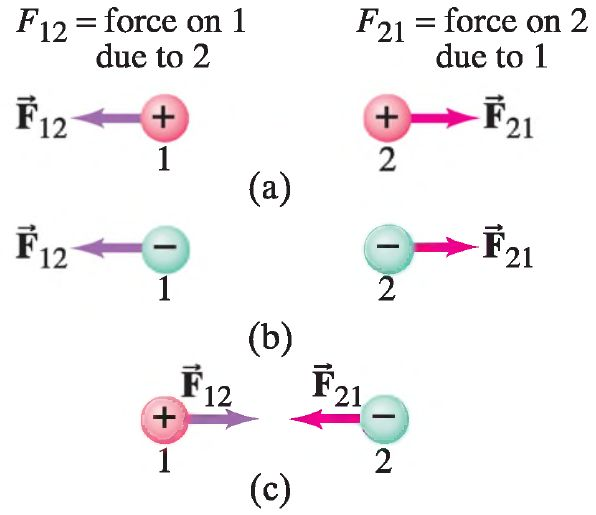
\includegraphics[height=1.7in]{images5/1.jpg}
\end{center}



   \column{2in}
\pause

\begin{equation}
\vec{F_{12}}=\frac{1}{4\pi \epsilon_0}\frac{Q_1Q_2}{r_{12}^2}\hat{r}_{12}
\end{equation}
\pause


Where $\epsilon_0$ is the permitivity of free space,
\pause

\begin{equation}
\epsilon_0=8.85\times10^{-12} \frac{C^2}{Nm^2}
\end{equation}



   \end{columns}






  \end{frame}

%%%%%%%%%%%%%%%%%%%%%%%%%%%%%%%%%%%%%%%%%%%%%%%%%%%%%%%%%%%%%%%%%%%



\begin{frame}
\frametitle{Electric Field}

1C $\rightarrow$ one Coulomb:

\vspace{3mm}
\pause

Amount of charge which, if placed on each of 2 point objects that are $1~m$ apart, result in a force of:


\vspace{3mm}
\pause

\begin{equation}
F=9\times 10^9 \frac{N\cdot m^2}{C^2}\frac{(1C)(1C)}{1~m^2}=9\times10^9~N
\end{equation}

\vspace{3mm}
\pause

Charge of one electron: $e=1.602\times 10^{-19}~C$

\vspace{3mm}
\pause

Elementary charge $\rightarrow$ smalest charge found in nature
\vspace{3mm}
\pause

charge $\propto n\cdot e$, $n$ integer, it is quantized.
  \end{frame}

%%%%%%%%%%%%%%%%%%%%%%%%%%%%%%%%%%%%%%%%%%%%%%%%%%%%%%%%%%%%%%%%%%%




\begin{frame}
\frametitle{Electric Field}

Electric field:

\begin{equation}
\vec{E}=\frac{\vec{F}}{q}
\end{equation}

\pause
\vspace{3mm}

$\vec{F}\rightarrow$ Force on a small positive test particle $q$.
\pause
\vspace{3mm}

\begin{equation}
[E]=\frac{N}{C}
\end{equation}
\pause
\vspace{3mm}

Then, the electric field generated by a charge $Q$ is:

\begin{equation}
E=\frac{1}{4\pi\epsilon_0}\frac{Q}{r^2}
\end{equation}


  \end{frame}

%%%%%%%%%%%%%%%%%%%%%%%%%%%%%%%%%%%%%%%%%%%%%%%%%%%%%%%%%%%%%%%%%%%




\begin{frame}
\frametitle{Electric Field}

Electric Field of more than one particle:
\pause
\vspace{3mm}



\begin{equation}
\vec{E}=\vec{E}_1+\vec{E}_2+\vec{E}_3+...
\end{equation}

\pause
\vspace{3mm}

Superposition principle.

  \end{frame}


%%%%%%%%%%%%%%%%%%%%%%%%%%%%%%%%%%%%%%%%%%%%%%%%%%%%%%%%%%%%%%%%%%%




\begin{frame}
\frametitle{Electric Field}

Electric Field of more than one particle:
\pause
\vspace{3mm}



\begin{equation}
\vec{E}=\vec{E}_1+\vec{E}_2+\vec{E}_3+...
\end{equation}

\pause
\vspace{3mm}

Superposition principle.

  \end{frame}



%%%%%%%%%%%%%%%%%%%%%%%%%%%%%%%%%%%%%%%%%%%%%%%%%%%%%%%%%%%%%%%%%%%



\begin{frame}
\frametitle{Electric Field}

Continuous charge distribution:

\pause

\begin{equation}
dE=\frac{1}{4\pi\epsilon_0}\frac{dQ}{r^2}, \ \ dQ=\rho dV
\end{equation}
\pause

\begin{equation}
\vec{E}=\int d\vec{E}
\end{equation}
\pause

\begin{equation}
E_x=\int dE cos\theta, \ \ E_y=\int dE sin\theta
\end{equation}

  \end{frame}



%%%%%%%%%%%%%%%%%%%%%%%%%%%%%%%%%%%%%%%%%%%%%%%%%%%%%%%%%%%%%%%%%%%






\begin{frame}
\frametitle{Electric Potential}

Work made by a constant force:

\begin{equation}
w=F\cdot d=q E d
\end{equation}

\pause

Potential Energy:

\begin{equation}
\Delta U = -w=- q E d
\end{equation}
\pause

Definition of  Electric Potential: Volt

\begin{equation}
V=\frac{U}{q}
\end{equation}



  \end{frame}



%%%%%%%%%%%%%%%%%%%%%%%%%%%%%%%%%%%%%%%%%%%%%%%%%%%%%%%%%%%%%%%%%%%


\begin{frame}
\frametitle{Electric Potential}

\begin{equation}
\Delta V=\frac{\Delta U}{q}=-\frac{w}{q}=-Ed
\end{equation}


\pause

Unit:

\begin{equation}
[V]=\frac{J}{C}
\end{equation}

\pause

In general,


\begin{equation}
\Delta V=-\int \vec{E}\cdot d \vec{\ell}
\end{equation}



  \end{frame}



%%%%%%%%%%%%%%%%%%%%%%%%%%%%%%%%%%%%%%%%%%%%%%%%%%%%%%%%%%%%%%%%%%%



\begin{frame}
\frametitle{Electric Flux}

Flux of a constant field through an area:
\pause

   \begin{columns}[c]
   \column{2in}  % slides are 3in high by 5in wide

    \begin{center}
  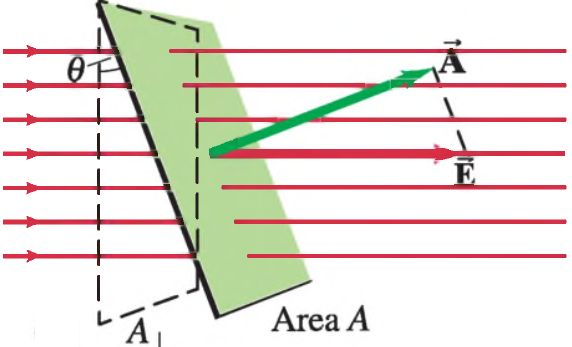
\includegraphics[height=1.2in]{images5/Eflux.jpg}
\end{center}

  
   \column{2in}



\begin{equation*}
\Phi_E=E\cdot A cos\theta=\vec{E}\cdot \vec{A}
\end{equation*}



   \end{columns}



  \end{frame}

%%%%%%%%%%%%%%%%%%%%%%%%%%%%%%%%%%%%%%%%%%%%%%%%%%%%%%%%%%%%%%%%%%%



\begin{frame}
\frametitle{Electric Flux}

Flux of a constant field through an area:
\pause

   \begin{columns}[c]
   \column{2in}  % slides are 3in high by 5in wide

    \begin{center}
  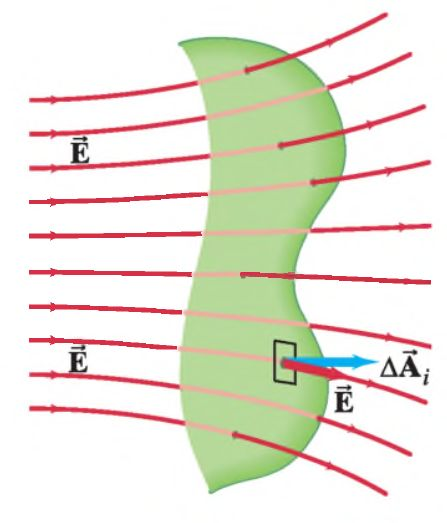
\includegraphics[height=1.2in]{images5/Eflux2.jpg}
\end{center}

  
   \column{2in}



General case,

\pause
\begin{equation*}
d\Phi_E=\vec{E}\cdot\vec{A}\rightarrow \Phi_E=\int \vec{E}\cdot\vec{A}
\end{equation*}


   \end{columns}



  \end{frame}

%%%%%%%%%%%%%%%%%%%%%%%%%%%%%%%%%%%%%%%%%%%%%%%%%%%%%%%%%%%%%%%%%%%

\begin{frame}
\frametitle{Electric Flux}

Electric flux through a closed surface.
\pause

   \begin{columns}[c]
   \column{2in}  % slides are 3in high by 5in wide

    \begin{center}
  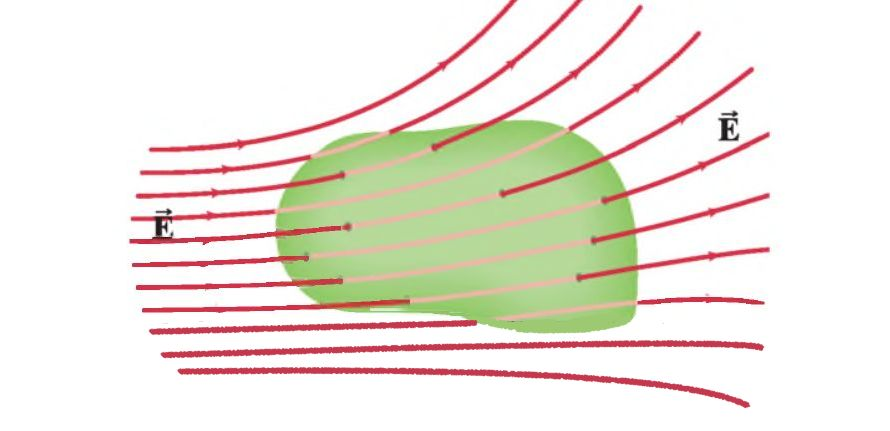
\includegraphics[height=1.in]{images5/Eflux3.jpg}
\end{center}

  
   \column{2in}



General case,

\pause
\begin{equation*}
\oint \vec{E}\cdot\vec{A}=0
\end{equation*}


   \end{columns}



  \end{frame}

%%%%%%%%%%%%%%%%%%%%%%%%%%%%%%%%%%%%%%%%%%%%%%%%%%%%%%%%%%%%%%%%%%%

\begin{frame}
\frametitle{Gaus Law}

Gaus Law: Relates the Electric Flux with the total charge enclosed inside a closed surface.
\pause

\begin{equation}
\oint \vec{E}\cdot d\vec{A}=\frac{Q}{\epsilon_0}
\end{equation}

\pause


Basically, this law says that if the flux crossing a closed surface is different from zero, then it is generated by a charge inside the surface.

  \end{frame}



%%%%%%%%%%%%%%%%%%%%%%%%%%%%%%%%%%%%%%%%%%%%%%%%%%%%%%%%%%%%%%%%%%%




\begin{frame}
\frametitle{Gaus Law}

Gaus $\rightarrow$ Coulomb
\vspace{3mm}
\pause

\
Consider a point charge enclosed into an sphere,
\vspace{3mm}
\pause

\begin{equation}
\oint \vec{E}\cdot d\vec{A}=E4\pi r^2\rightarrow E=\frac{1}{4\pi r^2}\frac{Q}{\epsilon_0}
\end{equation}

\pause
\vspace{3mm}

Coulomb $\rightarrow$ Gaus
\vspace{3mm}

\pause

\begin{equation}
\oint \vec{E}\cdot d\vec{A}=\oint \frac{1}{4\pi \epsilon_0} \frac{Q}{r^2}dA=\frac{Q}{4\pi r^2}4\pi r^2=\frac{Q}{\epsilon_0}
\end{equation}

  \end{frame}



%%%%%%%%%%%%%%%%%%%%%%%%%%%%%%%%%%%%%%%%%%%%%%%%%%%%%%%%%%%%%%%%%%%




\begin{frame}
\frametitle{Electric Current}

Electric Current: is generated by charge in motion.
\pause

\begin{equation}
I=\frac{dQ}{dt}
\end{equation}
\pause

\vspace{3mm}

Units:

\begin{equation*}
[I]=\frac{C}{s}= A,\ \ Ampere
\end{equation*}


  \end{frame}



%%%%%%%%%%%%%%%%%%%%%%%%%%%%%%%%%%%%%%%%%%%%%%%%%%%%%%%%%%%%%%%%%%%







\begin{frame}
\frametitle{Ohm's Law}

The Electric current in a wire is proportional to the  electric potential:
\pause
\vspace{3mm}

\begin{equation}
I=\frac{V}{R}
\end{equation}

\pause
\vspace{3mm}

where $R$ is the resistance, and it is due to the interaction of the electrons with the atoms in the wire.

\pause
\vspace{3mm}

Units:


\begin{equation}
[R]=\frac{V}{A}=\Omega,\ \ Ohm  
\end{equation}

  \end{frame}



%%%%%%%%%%%%%%%%%%%%%%%%%%%%%%%%%%%%%%%%%%%%%%%%%%%%%%%%%%%%%%%%%%%
\subsection{Magnetic Field}

\begin{frame}
\frametitle{Magnetic Field}



Sources of Magnetic Fields: Ampere's Law



   \begin{columns}[c]
   \column{2in}  % slides are 3in high by 5in wide
  

  \begin{center}
  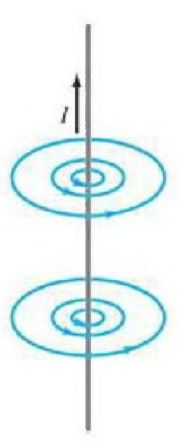
\includegraphics[height=1.5in]{images5/B.jpg}
\end{center}

\pause

The magnetic field generated by a straight wire is circular

   \column{2in}


\pause


\begin{equation*}
\oint \vec{B}\cdot d\vec{\ell}=\mu_0 I_{enclosed}
\end{equation*}

\pause

\begin{equation*}
\oint B d\ell=B 2\pi r=\mu_0I
\end{equation*}
\pause

\begin{equation}
\rightarrow=B =\frac{\mu_0I}{2\pi r}
\end{equation}

   \end{columns}




  \end{frame}

%%%%%%%%%%%%%%%%%%%%%%%%%%%%%%%%%%%%%%%%%%%%%%%%%%%%%%%%%%%%%%%%%%%


\begin{frame}
\frametitle{Magnetic Field}

The unit of the magnetic field is Tesla,

\begin{equation}
[B]=\frac{N}{A m}
\end{equation}

The constant $\mu_0$ is the \textbf{Vacuum Magnetic  Permeability}.

\begin{equation}
\mu_0=4\pi \times 10^{-7} \frac{T}{m A}
\end{equation}



  \end{frame}


%%%%%%%%%%%%%%%%%%%%%%%%%%%%%%%%%%%%%%%%%%%%%%%%%%%%%%%%%%%%%%%%%%%

\begin{frame}
\frametitle{Biot-Savat Law}


   \begin{columns}[c]
   \column{2in}  % slides are 3in high by 5in wide
  
\begin{center}
  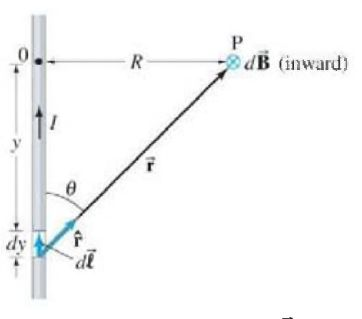
\includegraphics[height=1.5in]{images5/BS.jpg}
\end{center}

   \column{2in}
\begin{equation}
d\vec{B} =\frac{\mu_0}{4\pi}I \frac{d\vec{\ell}\times \hat{r}}{r^2}
\end{equation}

\pause
\begin{equation}
\rightarrow \vec{B} =\int\frac{\mu_0}{4\pi}I \frac{d\vec{\ell}\times \hat{r}}{r^2}
\end{equation}


   \end{columns}







  \end{frame}



%%%%%%%%%%%%%%%%%%%%%%%%%%%%%%%%%%%%%%%%%%%%%%%%%%%%%%%%%%%%%%%%%%%

\begin{frame}
\frametitle{Force due to a Magnetic Field}



Force on a current  due to a magnetic Field:
\vspace{3mm}

\pause
\begin{equation}
\vec{F}=I\vec{\ell}\times \vec{B}
\end{equation}
\pause
\vspace{3mm}

Force on a point charge  due to a magnetic Field:
\vspace{3mm}
\pause

\begin{equation}
\vec{F}=q\vec{v}\times \vec{B}
\end{equation}







  \end{frame}



%%%%%%%%%%%%%%%%%%%%%%%%%%%%%%%%%%%%%%%%%%%%%%%%%%%%%%%%%%%%%%%%%%%




\begin{frame}
\frametitle{Force due to a Magnetic Field}



Total force due to an electric and magnetic field:

\vspace{3mm}
\pause

\begin{equation}
\vec{F}=q(\vec{E}+\vec{v}\times \vec{B})\rightarrow Lorentz~Equation
\end{equation}






  \end{frame}


%%%%%%%%%%%%%%%%%%%%%%%%%%%%%%%%%%%%%%%%%%%%%%%%%%%%%%%%%%%%%%%%%%%

\begin{frame}

Example: Magnet
   \begin{columns}[c]
   \column{2in}  % slides are 3in high by 5in wide

  \begin{center}
  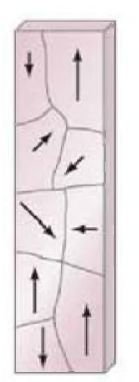
\includegraphics[height=1.5in]{images5/ferromagnetic.jpg}
\end{center}


   \column{2in}

\pause



In some materials called \textbf{Ferromagnetic}, the angular momentum of electrons are aligned so that they create a resultant macroscopic magnetic field.

\vspace{3mm}

\pause

Iron - Cobalt - Nickel

   \end{columns}









  \end{frame}



%%%%%%%%%%%%%%%%%%%%%%%%%%%%%%%%%%%%%%%%%%%%%%%%%%%%%%%%%%%%%%%%%%%
\subsection{Electromagnetic Radiation}

\begin{frame}

When the electric and magnetic fields are static, the are separate entities. But when they are changing,  we can not treat them separately 

\pause
\vspace{3mm}

$\rightarrow$ \textbf{Maxwell Equations}

\pause
\vspace{3mm}

A changing magnetic field generates a changing electric field that generates a changing magnetic field.

\pause
\vspace{3mm}

$\rightarrow$ \textbf{Wave traveling in the espace}

  \end{frame}

%%%%%%%%%%%%%%%%%%%%%%%%%%%%%%%%%%%%%%%%%%%%%%%%%%%%%%%%%%%%%%%%%%%


\begin{frame}
\frametitle{Maxwell Equations}


  \begin{center}
  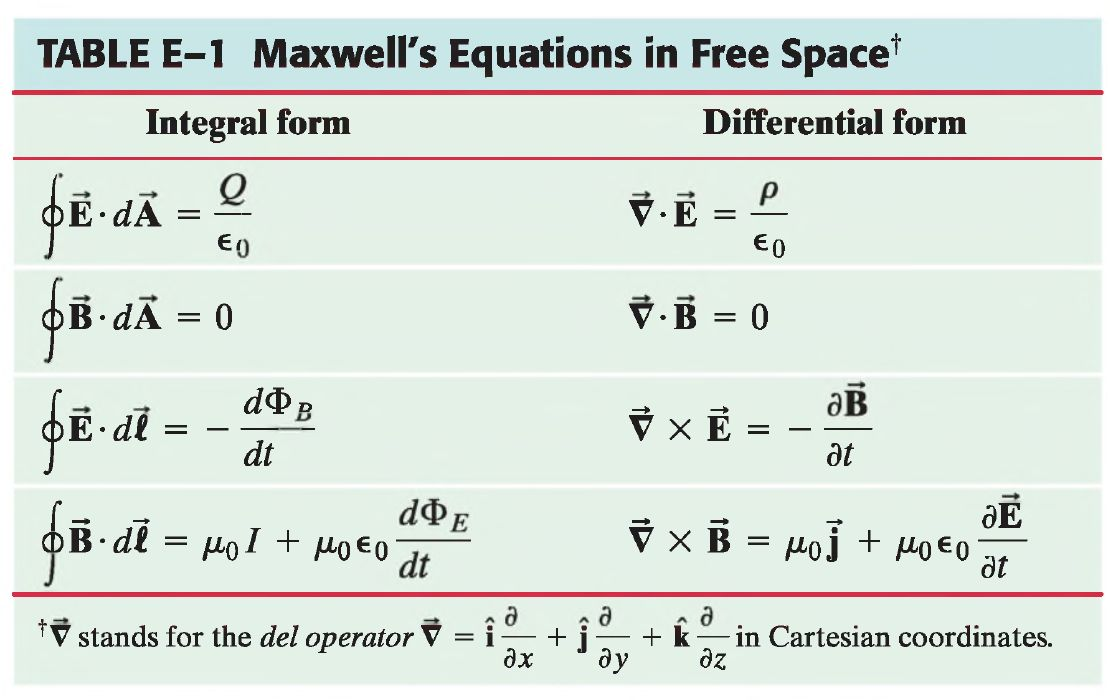
\includegraphics[height=2.3in]{images5/Maxwell_EQ.jpg}
\end{center}



  \end{frame}



%%%%%%%%%%%%%%%%%%%%%%%%%%%%%%%%%%%%%%%%%%%%%%%%%%%%%%%%%%%%%%%%%%%



\begin{frame}


   \begin{columns}[c]
   \column{2in}  % slides are 3in high by 5in wide
  
  \begin{center}
  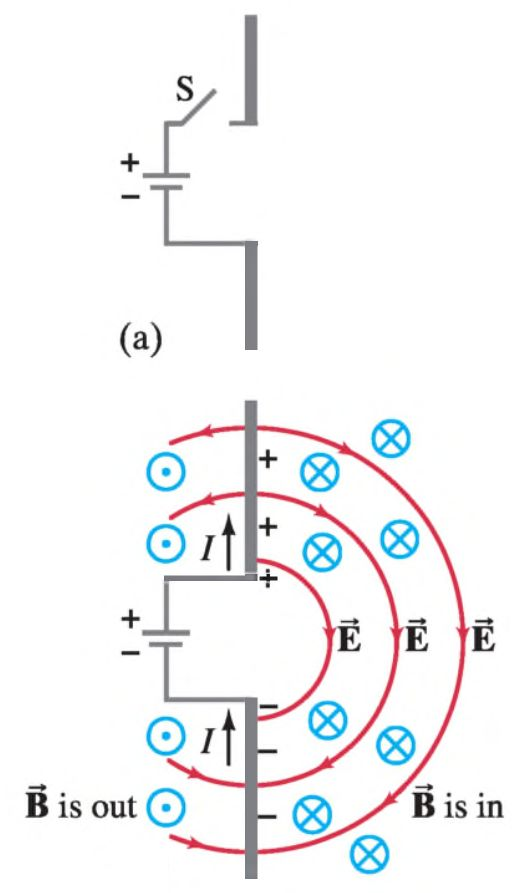
\includegraphics[height=2.3in]{images5/antenna1.jpg}
\end{center}


   \column{2.7in}


\begin{itemize}
\pause
\item We connect two rod to a battery $\rightarrow$ Electric Field 
\pause
\item  The charge is re-distributed $\rightarrow$  Magnetic field 

\end{itemize}

   \end{columns}


  \end{frame}


%%%%%%%%%%%%%%%%%%%%%%%%%%%%%%%%%%%%%%%%%%%%%%%%%%%%%%%%%%%%%%%%%%%



\begin{frame}


   \begin{columns}[c]
   \column{2in}  % slides are 3in high by 5in wide
  
  \begin{center}
  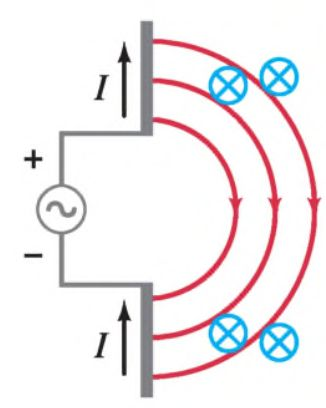
\includegraphics[height=1.7in]{images5/antenna2.jpg}
\end{center}


   \column{2.7in}


\begin{itemize}
\pause
\item sinusoidal voltage   $\rightarrow$ Alternating Current
\pause
\item $\rightarrow$ variable Electric and Magnetic Fields.
\end{itemize}

   \end{columns}


  \end{frame}


%%%%%%%%%%%%%%%%%%%%%%%%%%%%%%%%%%%%%%%%%%%%%%%%%%%%%%%%%%%%%%%%%%%






\begin{frame}


   \begin{columns}[c]
   \column{2in}  % slides are 3in high by 5in wide
  
  \begin{center}
  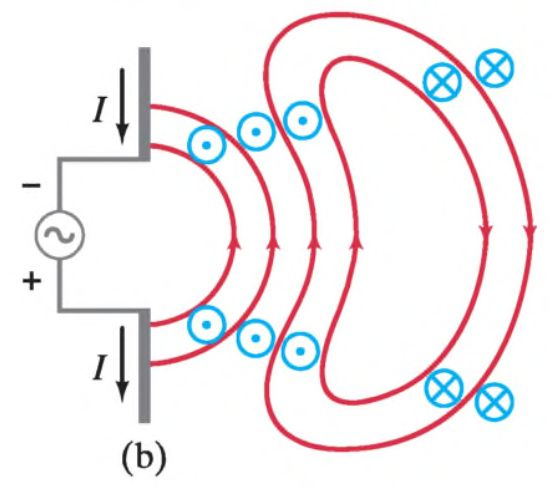
\includegraphics[height=1.7in]{images5/antenna3.jpg}
\end{center}


   \column{2.7in}


\begin{itemize}
\pause
\item Old Field lines fold back to connect to some of the new lines $\rightarrow$ closed loops
\pause
 \item The old field don't suddenly disappear
\pause
 \item changing EF $\rightarrow$ changing MF $\rightarrow$ changing EF ...$\rightarrow$ so on
\pause
 \item This combination of  changing EF and MF moving outward is self supporting, no longer depending on the antenna. 
\pause
 \item They are on their way to distant points.

\end{itemize}

   \end{columns}


  \end{frame}

%%%%%%%%%%%%%%%%%%%%%%%%%%%%%%%%%%%%%%%%%%%%%%%%%%%%%%%%%%%%%%%%%%%



\begin{frame}
\frametitle{Characteristics of Electromagnetic Waves}

\begin{itemize}

\item The field not far the antenna (\textit{Near Field}) is complicated.
\pause

\item The field far from the antenna (\textit{Far Field}) is quite flat $\rightarrow$ Plane Waves
\pause

\item The field also travels in other directions, the strength is greater in the direction perpendicular to the antenna.
\pause

\item The magnitude of $\vec{E}$ and $\vec{B}$ decreases with distance as $1/r$.
\pause

\item $\vec{E}\perp\vec{B}$, and they are $\perp$ to the direction of propagation.
\pause

\item  of $\vec{E}$ and $\vec{B}$ are in phase.

\end{itemize}

  \end{frame}


%%%%%%%%%%%%%%%%%%%%%%%%%%%%%%%%%%%%%%%%%%%%%%%%%%%%%%%%%%%%%%%%%%%



\begin{frame}
\frametitle{ Electromagnetic Waves}


 \begin{center}
  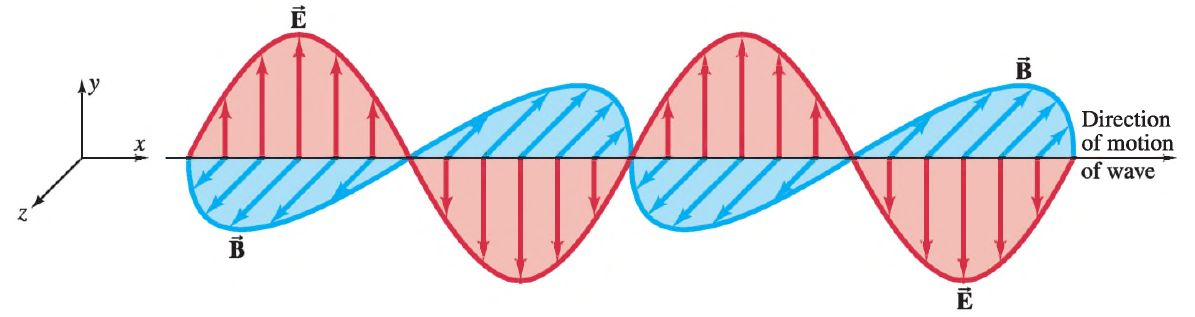
\includegraphics[height=0.6in]{images5/EMwave.jpg}
\end{center}


\begin{itemize}

 

\item Transverse wave
\pause 
\item Waves of field, not of matter
\pause
\item EM waves can propagate in empty space.

\pause
\vspace{3mm}
\pause

EM waves are produced by electric charges that are oscillating $\rightarrow$ are undergoing into acceleration in general.
\pause
\vspace{3mm}

\textbf{Accelerated electric charges give rise to electromagnetic waves}

\end{itemize}

  \end{frame}







%%%%%%%%%%%%%%%%%%%%%%%%%%%%%%%%%%%%%%%%%%%%%%%%%%%%%%%%%%%%%%%%%%%


\begin{frame}
\frametitle{Mathematical Description}

\begin{itemize}
\item Let's consider a region of free space where there are no charges or conduction currents, $Q=0, I=0$
\pause 
\item Plane waves
\pause
\item Waves traveling in the x-direction, $\vec{v}=v\hat{\imath}$
\end{itemize}


  \end{frame}


%%%%%%%%%%%%%%%%%%%%%%%%%%%%%%%%%%%%%%%%%%%%%%%%%%%%%%%%%%%%%%%%%%%



\begin{frame}
\frametitle{Mathematical Description}


The Maxwell equation take the form:


 \begin{center}
  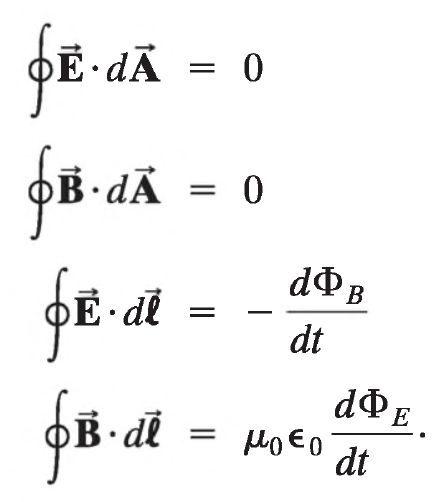
\includegraphics[height=1.7in]{images5/Maxwell_EQ2.jpg}
\end{center}


  \end{frame}




%%%%%%%%%%%%%%%%%%%%%%%%%%%%%%%%%%%%%%%%%%%%%%%%%%%%%%%%%%%%%%%%%%%


\begin{frame}


We describe the waves as sinusoidal waves with wavelength $\lambda$ and frequency $f$:
\pause
\vspace{3mm}


\begin{eqnarray}
E=E_y&=&E_0sin(kx-\omega t)\\
B=B_z&=&B_0sin(kx-\omega t)
\end{eqnarray}
\pause
\vspace{3mm}

where,
\pause



\begin{equation*}
k=\frac{2\pi}{\lambda},\ \ \omega=2\pi f,\ \ f\lambda=\frac{\omega}{k}=v
\end{equation*}


  \end{frame}



%%%%%%%%%%%%%%%%%%%%%%%%%%%%%%%%%%%%%%%%%%%%%%%%%%%%%%%%%%%%%%%%%%%


\begin{frame}

\frametitle{Speed of light}



   \begin{columns}[c]
   \column{2in}  % slides are 3in high by 5in wide
  

 \begin{center}
  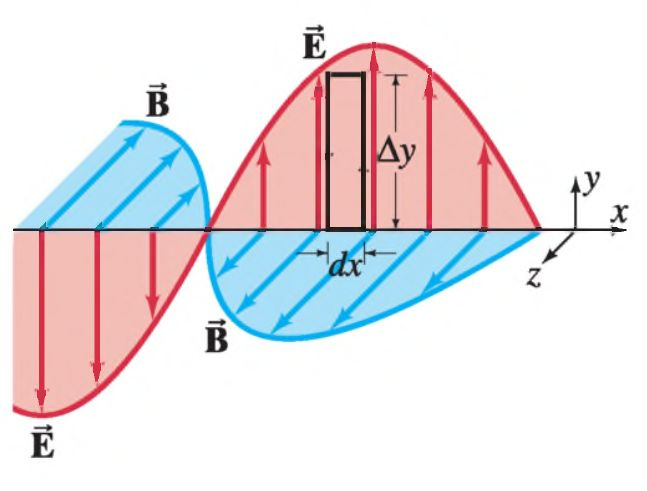
\includegraphics[height=1.4in]{images5/EMwave2.jpg}
\end{center}


   \column{2.5in}
\pause


\begin{equation*}
\oint \vec{E}d\vec{\ell}=\frac{-d\Phi_B}{dt}
\end{equation*}

\pause 

\begin{equation*}
\oint \vec{E}d\vec{\ell}=(E+dE)\Delta y-E\Delta y=dE\Delta y
\end{equation*}
\pause

\begin{equation*}
\rightarrow dE\Delta y=\frac{-d\Phi_B}{dt}
\end{equation*}


   \end{columns}




  \end{frame}











%%%%%%%%%%%%%%%%%%%%%%%%%%%%%%%%%%%%%%%%%%%%%%%%%%%%%%%%%%%%%%%%%%%


\begin{frame}

\frametitle{Speed of light}



   \begin{columns}[c]
   \column{2in}  % slides are 3in high by 5in wide
  
 \begin{center}
  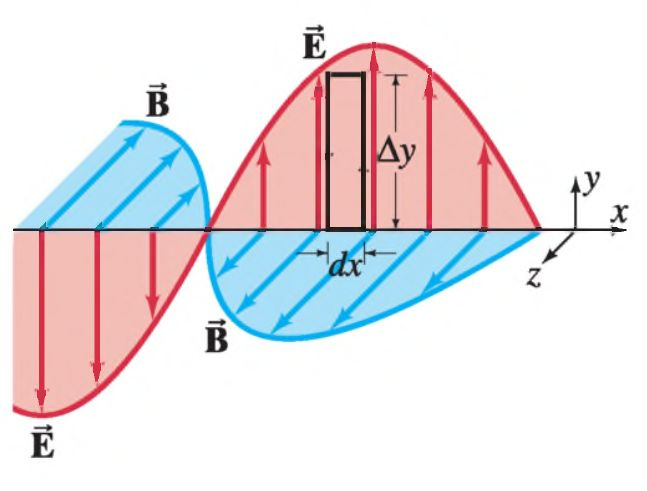
\includegraphics[height=1.4in]{images5/EMwave2.jpg}
\end{center}


   \column{2.5in}
\pause

The flux is,

\begin{equation*}
\Phi_B=BdA=Bdx\Delta y
\end{equation*}

\pause

\begin{equation*}
\rightarrow dE\Delta y=-\frac{dB}{dt}dx\Delta y
\end{equation*}
\pause

\begin{equation}
\rightarrow \frac{dE}{dx}=-\frac{dB}{dt}\rightarrow  \frac{\partial E}{\partial x}=-\frac{\partial B}{\partial t}
\label{eq:1}
\end{equation}




   \end{columns}




  \end{frame}









%%%%%%%%%%%%%%%%%%%%%%%%%%%%%%%%%%%%%%%%%%%%%%%%%%%%%%%%%%%%%%%%%%%


\begin{frame}

\frametitle{Speed of light}



   \begin{columns}[c]
   \column{2in}  % slides are 3in high by 5in wide
  
 \begin{center}
  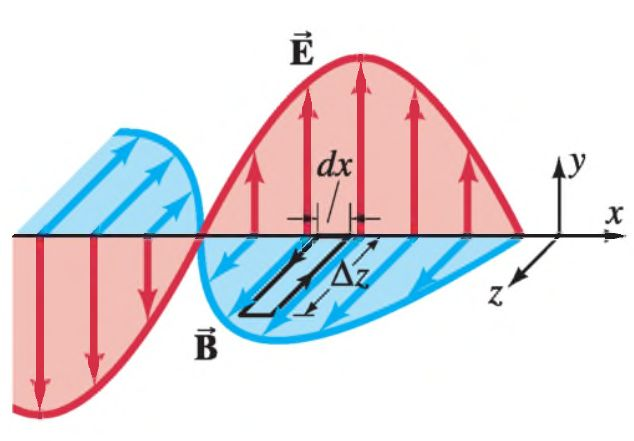
\includegraphics[height=1.4in]{images5/EMwave3.jpg}
\end{center}


   \column{2.5in}
\pause

The same with 

\begin{equation*}
\oint \vec{B}d\vec{\ell}=\mu_0\epsilon_0\frac{d\Phi_E}{dt}
\end{equation*}
\pause

\begin{equation*}
\rightarrow   \oint \vec{B}d\vec{\ell}=-(B+dB)\Delta y + B\delta y
\end{equation*}
\pause

\begin{equation*}
\rightarrow   \oint \vec{B}d\vec{\ell}=-dB\Delta y
\end{equation*}
\pause



   \end{columns}




  \end{frame}







%%%%%%%%%%%%%%%%%%%%%%%%%%%%%%%%%%%%%%%%%%%%%%%%%%%%%%%%%%%%%%%%%%%


\begin{frame}

\frametitle{Speed of light}






\begin{equation}
\rightarrow  \frac{\partial B}{\partial x}=-\mu_0\epsilon_0 \frac{\partial E}{\partial t}
\label{eq:2}
\end{equation}

\pause
\vspace{3mm}

using the equation (\ref{eq:1}) and the expression for $E(x,t)$ and $B(x,t)$,
\pause

\begin{equation*}
\frac{E_0}{B_0}=\frac{\omega}{k}=v
\end{equation*}
\pause

$E$ and $B$ are in phase,

\pause

\begin{equation*}
\rightarrow \frac{E}{B}=v
\end{equation*}

  \end{frame}







%%%%%%%%%%%%%%%%%%%%%%%%%%%%%%%%%%%%%%%%%%%%%%%%%%%%%%%%%%%%%%%%%%%


\begin{frame}

\frametitle{Speed of light}



Using the equation (\ref{eq:2}) and the expression for $E(x,t)$ and $B(x,t)$,
\pause

\begin{equation*}
\frac{E_0}{B_0}=\frac{k}{\mu_0\epsilon_0\omega}
\end{equation*}
\pause



\begin{equation*}
\rightarrow v=\frac{1}{\mu_0\epsilon_0}\frac{1}{v}
\end{equation*}



  \end{frame}






%%%%%%%%%%%%%%%%%%%%%%%%%%%%%%%%%%%%%%%%%%%%%%%%%%%%%%%%%%%%%%%%%%%


\begin{frame}

\frametitle{Speed of light}



Then, the velocity of propagation of the wave is,

\begin{equation}
v^2=\frac{1}{\epsilon_0\mu_0}\rightarrow v=\frac{1}{\sqrt{\epsilon_0 \mu_0}}=c
\end{equation}

$c$ is the speed of light,

\begin{equation}
c=3\times 10^8~ m/s
\end{equation}

  \end{frame}




%%%%%%%%%%%%%%%%%%%%%%%%%%%%%%%%%%%%%%%%%%%%%%%%%%%%%%%%%%%%%%%%%%%


\begin{frame}

\frametitle{Wave Equation}

We can derive the speed of light without assuming sinusoidal waves...
\pause
\vspace{3mm}

\begin{eqnarray*}
  \frac{\partial E}{\partial x}&=&-\frac{\partial B}{\partial t}\\
 \frac{\partial B}{\partial x}&=&-\mu_0\epsilon_0 \frac{\partial E}{\partial t}
\end{eqnarray*}

\pause

\begin{equation}
\rightarrow \frac{\partial^2 E}{\partial x^2}=-\frac{\partial^2 B }{\partial x\partial t}=\mu_0\epsilon_0\frac{\partial^2 E}{\partial^2 t}
\end{equation}


  \end{frame}




%%%%%%%%%%%%%%%%%%%%%%%%%%%%%%%%%%%%%%%%%%%%%%%%%%%%%%%%%%%%%%%%%%%


\begin{frame}

\frametitle{Wave Equation}



\begin{equation}
\rightarrow \frac{\partial^2 E}{\partial x^2}=\mu_0\epsilon_0\frac{\partial^2 E}{\partial^2 t}
\end{equation}
\pause

this is the wave equation for a wave that is traveling at a speed,
\pause

\begin{equation*}
\frac{1}{v^2}=\mu_0\epsilon_0\rightarrow v=\frac{1}{\sqrt{\epsilon_0 \mu_0}}
\end{equation*}
\pause
Using the another eq. we obtain the equaiton for $B$,
\pause

\begin{equation}
\frac{\partial^2 B}{\partial x^2}=\mu_0\epsilon_0\frac{\partial^2 B}{\partial^2 t}
\end{equation}



  \end{frame}


%%%%%%%%%%%%%%%%%%%%%%%%%%%%%%%%%%%%%%%%%%%%%%%%%%%%%%%%%%%%%%%%%%%


\begin{frame}

\frametitle{Measuring the speed of light}

Michelson's Experiment

  \begin{center}
  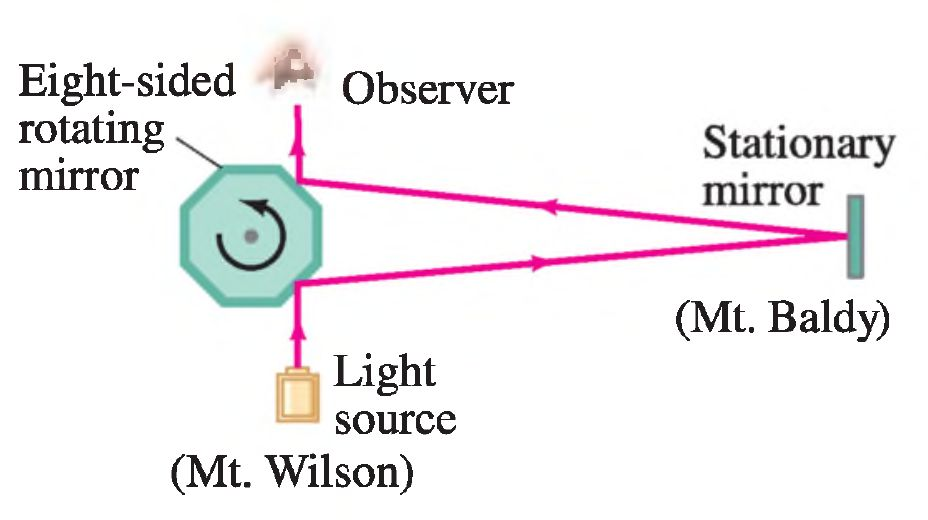
\includegraphics[height=2.0in]{images5/Michelson.jpg}
\end{center}




  \end{frame}

%%%%%%%%%%%%%%%%%%%%%%%%%%%%%%%%%%%%%%%%%%%%%%%%%%%%%%%%%%%%%%%%%%%


\begin{frame}

\frametitle{Electromagnetic spectrum}

The frequency of light is related with its speed thought the expression,

\begin{equation*}
c=f\lambda
\end{equation*}

  \begin{center}
  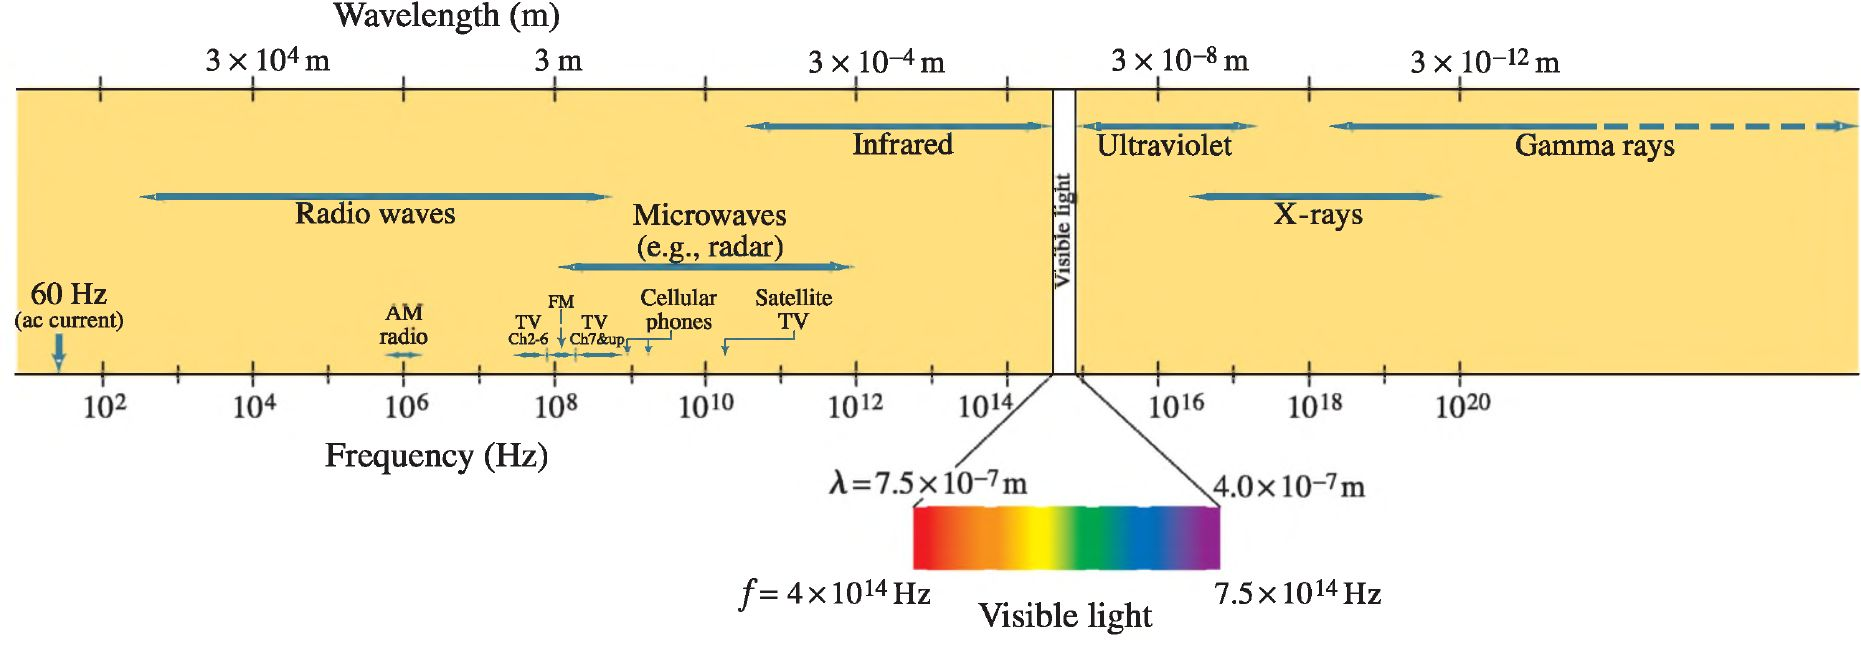
\includegraphics[height=1.5in]{images5/spectrum.jpg}
\end{center}



  \end{frame}


%%%%%%%%%%%%%%%%%%%%%%%%%%%%%%%%%%%%%%%%%%%%%%%%%%%%%%%%%%%%%%%%%%%


\begin{frame}

\frametitle{Electromagnetic spectrum}

The frequency of light is related with its speed thought the expression,

\begin{equation*}
c=f\lambda
\end{equation*}

  \begin{center}
  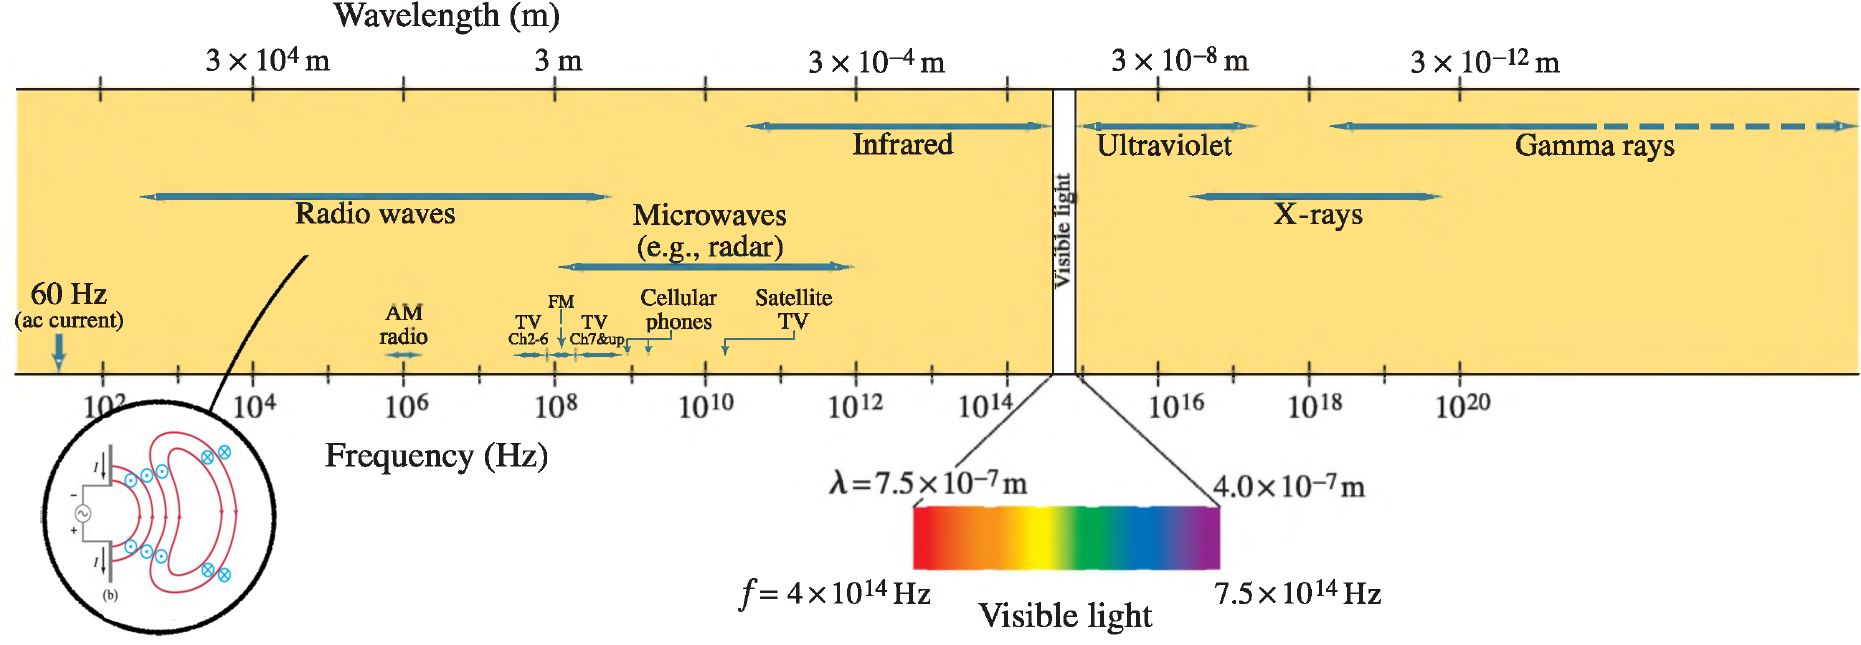
\includegraphics[height=1.5in]{images5/spectrum2.jpg}
\end{center}



  \end{frame}

%%%%%%%%%%%%%%%%%%%%%%%%%%%%%%%%%%%%%%%%%%%%%%%%%%%%%%%%%%%%%%%%%%%


\begin{frame}

\frametitle{Electromagnetic spectrum}

The frequency of light is related with its speed thought the expression,

\begin{equation*}
c=f\lambda
\end{equation*}

  \begin{center}
  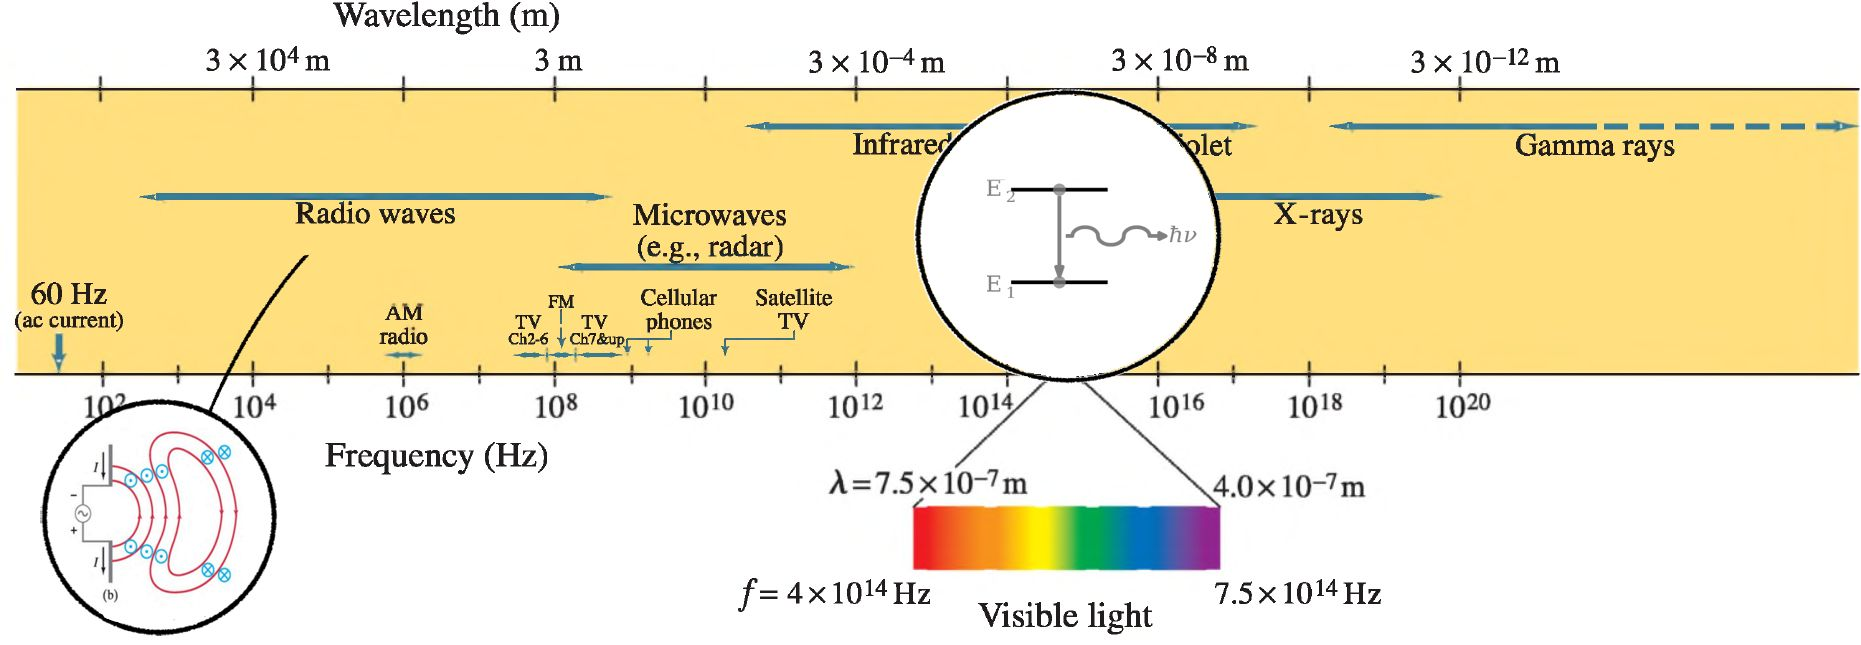
\includegraphics[height=1.5in]{images5/spectrum3.jpg}
\end{center}



  \end{frame}

%%%%%%%%%%%%%%%%%%%%%%%%%%%%%%%%%%%%%%%%%%%%%%%%%%%%%%%%%%%%%%%%%%%


\begin{frame}

\frametitle{Electromagnetic spectrum}

The frequency of light is related with its speed thought the expression,

\begin{equation*}
c=f\lambda
\end{equation*}

  \begin{center}
  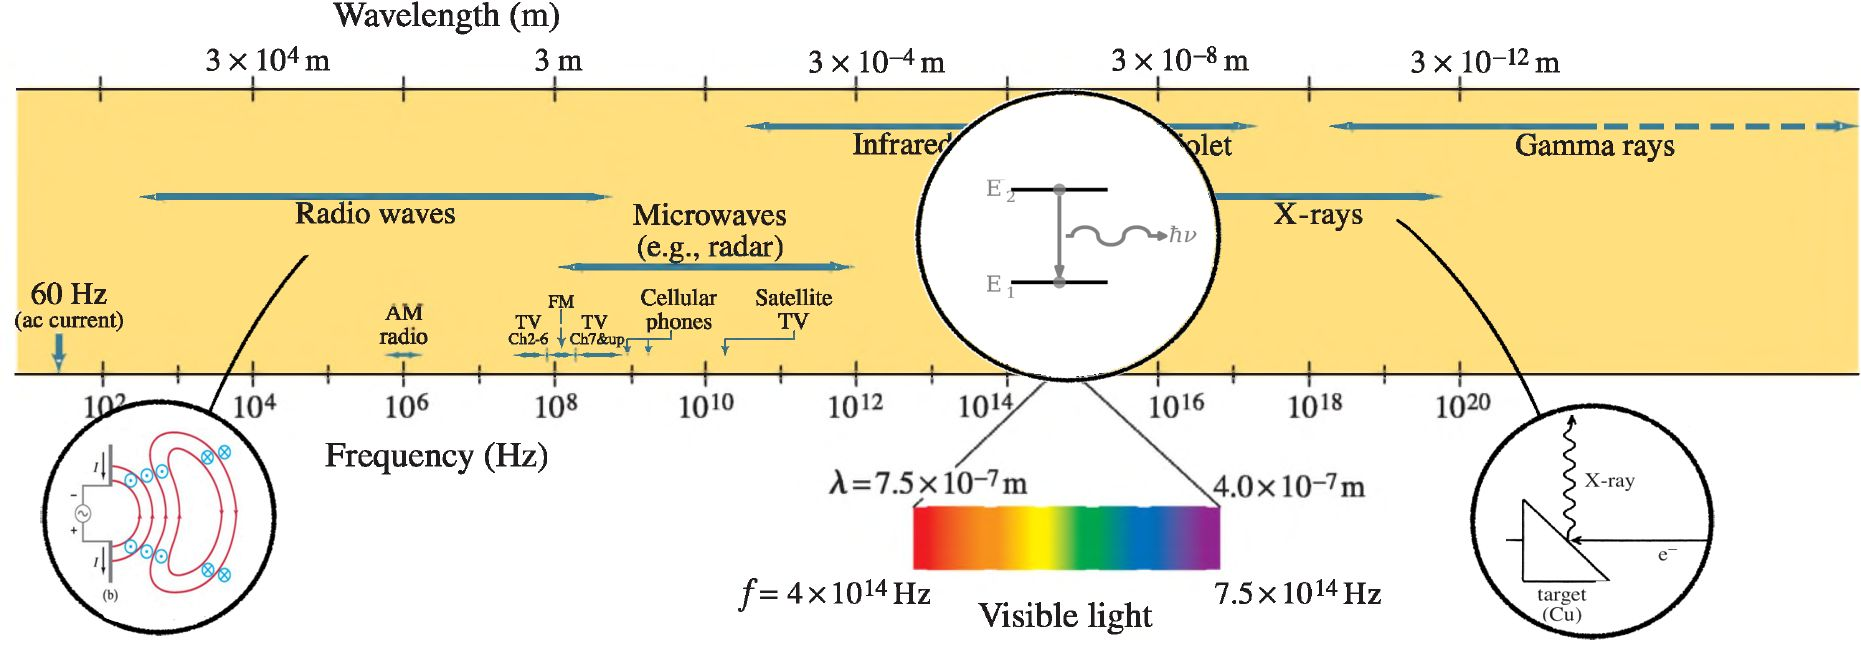
\includegraphics[height=1.5in]{images5/spectrum4.jpg}
\end{center}



  \end{frame}

%%%%%%%%%%%%%%%%%%%%%%%%%%%%%%%%%%%%%%%%%%%%%%%%%%%%%%%%%%%%%%%%%%%


\begin{frame}

\frametitle{Electromagnetic spectrum}

The frequency of light is related with its speed thought the expression,

\begin{equation*}
c=f\lambda
\end{equation*}

  \begin{center}
  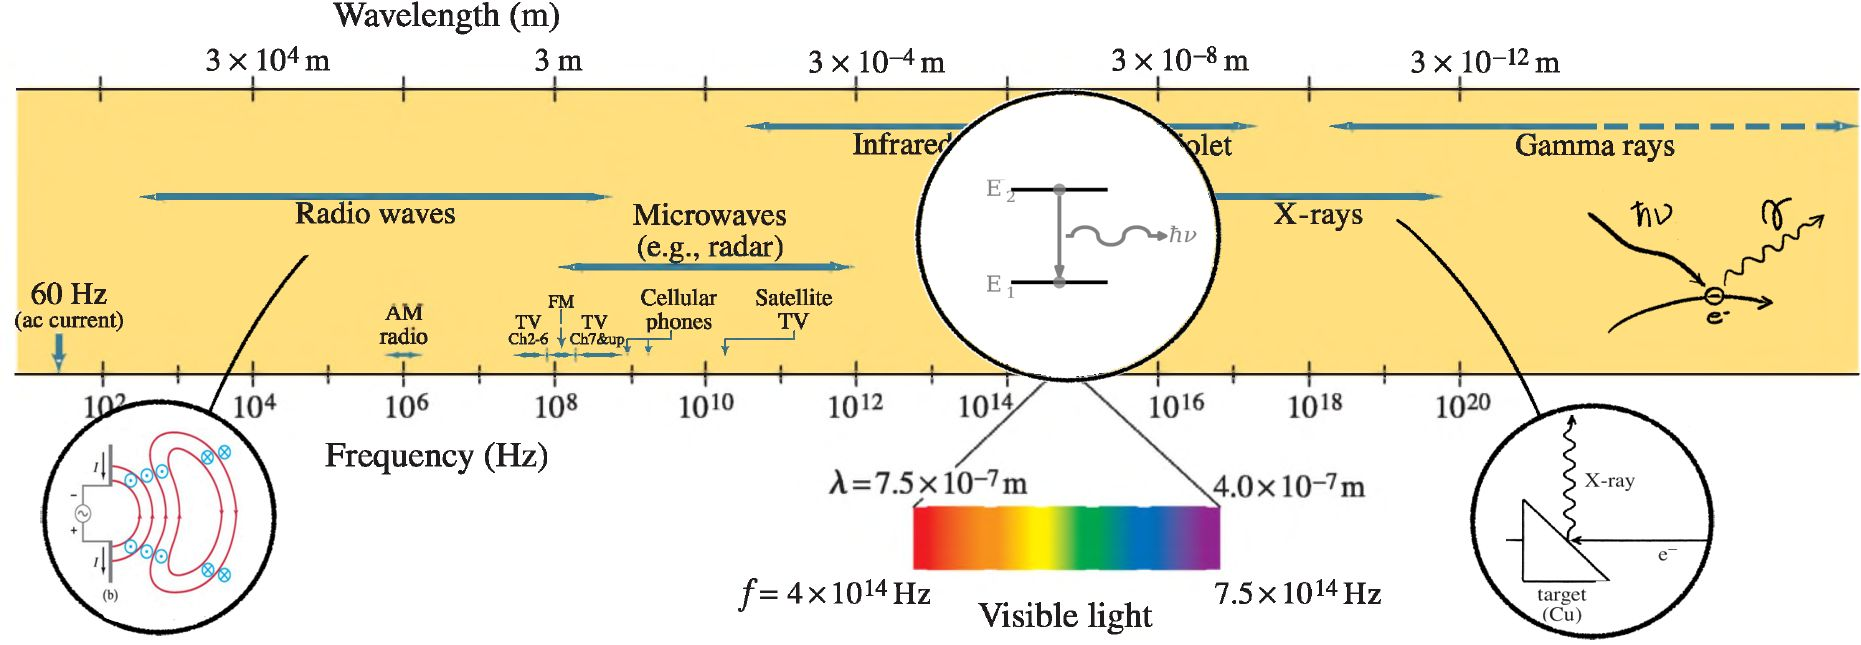
\includegraphics[height=1.5in]{images5/spectrum5.jpg}
\end{center}



  \end{frame}



%%%%%%%%%%%%%%%%%%%%%%%%%%%%%%%%%%%%%%%%%%%%%%%%%%%%%%%%%%%%%%%%%%%


\begin{frame}

\frametitle{Electromagnetic spectrum}

Example:

\vspace{3mm}

BB radiation $\rightarrow I\propto \frac{1}{e^{\frac{\hbar \nu}{kT}}-1}$

\vspace{3mm}

Synchrotron radiation $\rightarrow \nu^{\alpha}$ Power Law


  \end{frame}

%%%%%%%%%%%%%%%%%%%%%%%%%%%%%%%%%%%%%%%%%%%%%%%%%%%%%%%%%%%%%%%%%%%


\begin{frame}

\frametitle{Electromagnetic spectrum}

Application: knowing what process are occurring in an Astrophysical Object.

  \begin{center}
  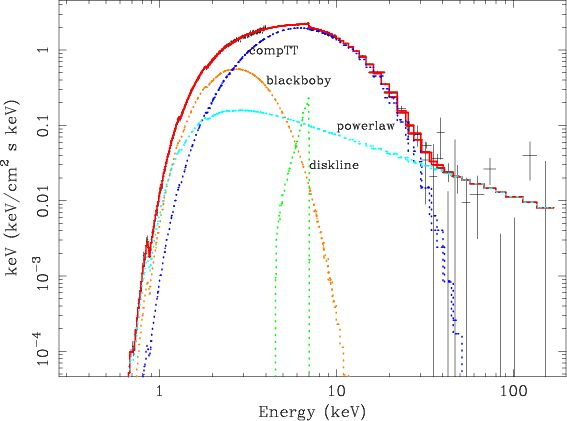
\includegraphics[height=2.0in]{images5/NSspectrum.jpg}
\end{center}



  \end{frame}





%%%%%%%%%%%%%%%%%%%%%%%%%%%%%%%%%%%%%%%%%%%%%%%%%%%%%%%%%%%%%%%%%%%


\begin{frame}

\frametitle{Huygens' principle}

\textit{Every point on a wave front can be considered as a source o f tiny
wavelets that spread out in the forward direction at the speed o f the wave itself
The new wave front is the envelope o f all the wavelets— that is, the tangent to all
o f them.}

  \begin{center}
  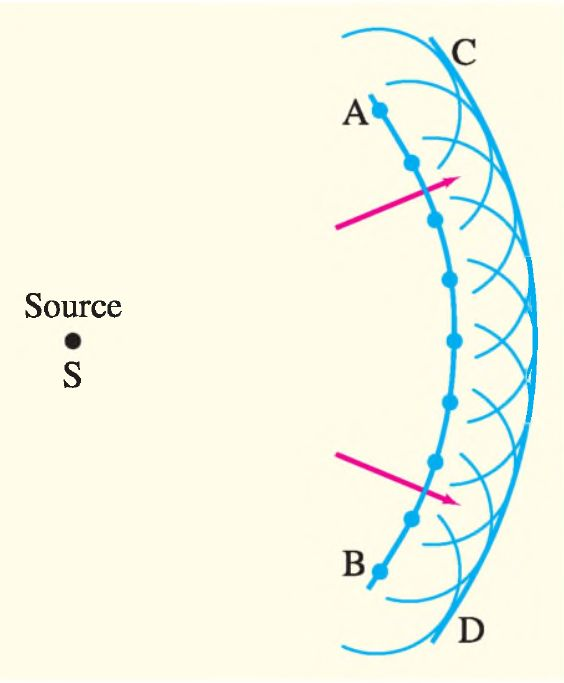
\includegraphics[height=1.3in]{images5/Huygen.jpg}
\end{center}



  \end{frame}




%%%%%%%%%%%%%%%%%%%%%%%%%%%%%%%%%%%%%%%%%%%%%%%%%%%%%%%%%%%%%%%%%%%


\begin{frame}

\frametitle{Diffraction}





   \begin{columns}[c]
   \column{2.8in}  % slides are 3in high by 5in wide

  What happens when waves impinge on an obstacle?
\pause


 $\rightarrow$ waves bend in behind an obstacle
\pause
\vspace{3mm}

 $\rightarrow$The bending into the "shadow region" is known as diffraction
\pause

\vspace{3mm}

 $\rightarrow$ If the opening is much larger then than the wavelength, diffraction goes unnoticed. 
\pause



   \column{1.4in}

  \begin{center}
  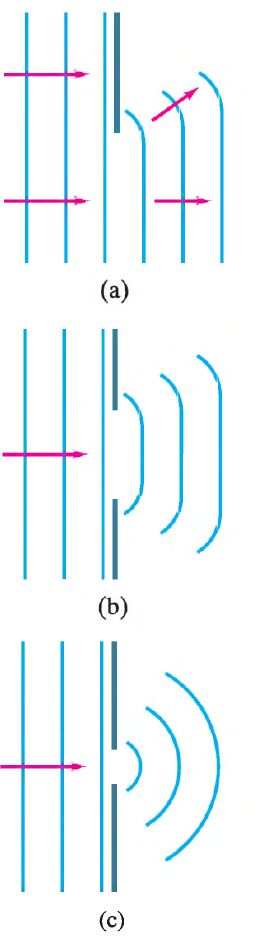
\includegraphics[height=2.3in]{images5/diffraction.jpg}
\end{center}

   \end{columns}




  \end{frame}




%%%%%%%%%%%%%%%%%%%%%%%%%%%%%%%%%%%%%%%%%%%%%%%%%%%%%%%%%%%%%%%%%%%


\begin{frame}

\frametitle{Refraction}

What happens when a waves front changes the medium?
\pause

  \begin{center}
  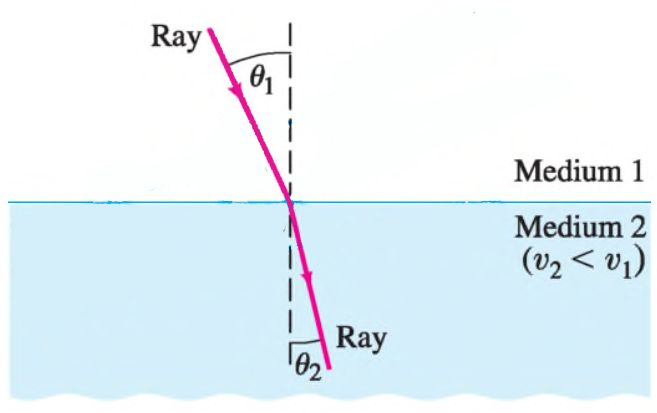
\includegraphics[height=1.8in]{images5/Refraction0.jpg}
\end{center}






  \end{frame}





%%%%%%%%%%%%%%%%%%%%%%%%%%%%%%%%%%%%%%%%%%%%%%%%%%%%%%%%%%%%%%%%%%%


\begin{frame}

\frametitle{Refraction}

We are going to use the Huygens' principle to explain this...
\pause





   \begin{columns}[c]
   \column{2in}  % slides are 3in high by 5in wide

    \begin{center}
  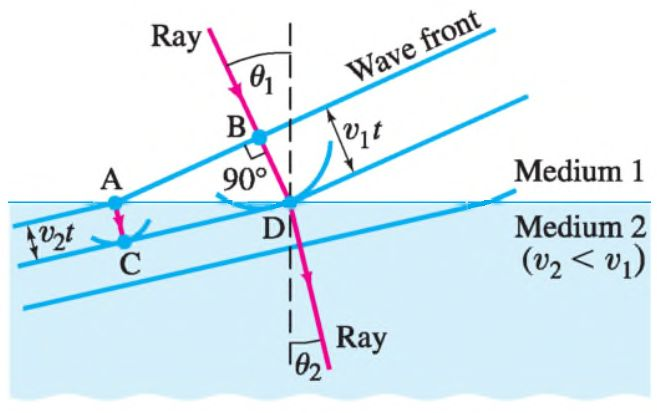
\includegraphics[height=1.5in]{images5/Refraction.jpg}
\end{center}


   \column{2in}

\pause

\begin{equation*}
sin\theta_1=\frac{v_1 t}{AD},\ \ sin\theta_2=\frac{v_2 t }{AD}
\end{equation*}

\pause


\begin{equation*}
\rightarrow \frac{sin\theta_1}{sin\theta_2}=\frac{v_1}{v_2}
\end{equation*}




   \end{columns}


  \end{frame}




%%%%%%%%%%%%%%%%%%%%%%%%%%%%%%%%%%%%%%%%%%%%%%%%%%%%%%%%%%%%%%%%%%%


\begin{frame}

\frametitle{Refraction}



The frequency does not change, but the wavelength does,

\pause

\begin{equation*}
 \frac{\lambda_2}{\lambda_1}=\frac{v_2}{v_1}=\frac{n_1}{n_2}
\end{equation*}
\pause

where,

\begin{equation}
n=\frac{c}{v}
\end{equation}
\pause
\vspace{3mm}

is the \textbf{refraction index}.


  \end{frame}


%%%%%%%%%%%%%%%%%%%%%%%%%%%%%%%%%%%%%%%%%%%%%%%%%%%%%%%%%%%%%%%%%%%


\begin{frame}

\frametitle{Refraction}


Why the velocity change?
\pause

\begin{equation}
v=\frac{1}{\sqrt{\epsilon \mu}}
\end{equation}


$\mu\rightarrow$ The resistance of a material to be penetrated by a magnetic field.

\pause
\vspace{3mm}

$\epsilon\rightarrow$ The resistance of a material to be penetrated by an electric field.



  \end{frame}


%%%%%%%%%%%%%%%%%%%%%%%%%%%%%%%%%%%%%%%%%%%%%%%%%%%%%%%%%%%%%%%%%%%


\begin{frame}

\frametitle{Refraction}


Why the velocity change?
\pause

\begin{equation}
v=\frac{1}{\sqrt{\epsilon \mu}}
\end{equation}


$\mu\rightarrow$ The resistance of a material to be penetrated by a magnetic field.

\pause
\vspace{3mm}

$\epsilon\rightarrow$ The resistance of a material to be penetrated by an electric field.



  \end{frame}





%%%%%%%%%%%%%%%%%%%%%%%%%%%%%%%%%%%%%%%%%%%%%%%%%%%%%%%%%%%%%%%%%%%


\begin{frame}

\frametitle{Refraction}


Example: Mirages

\vspace{3mm}

  \begin{center}
  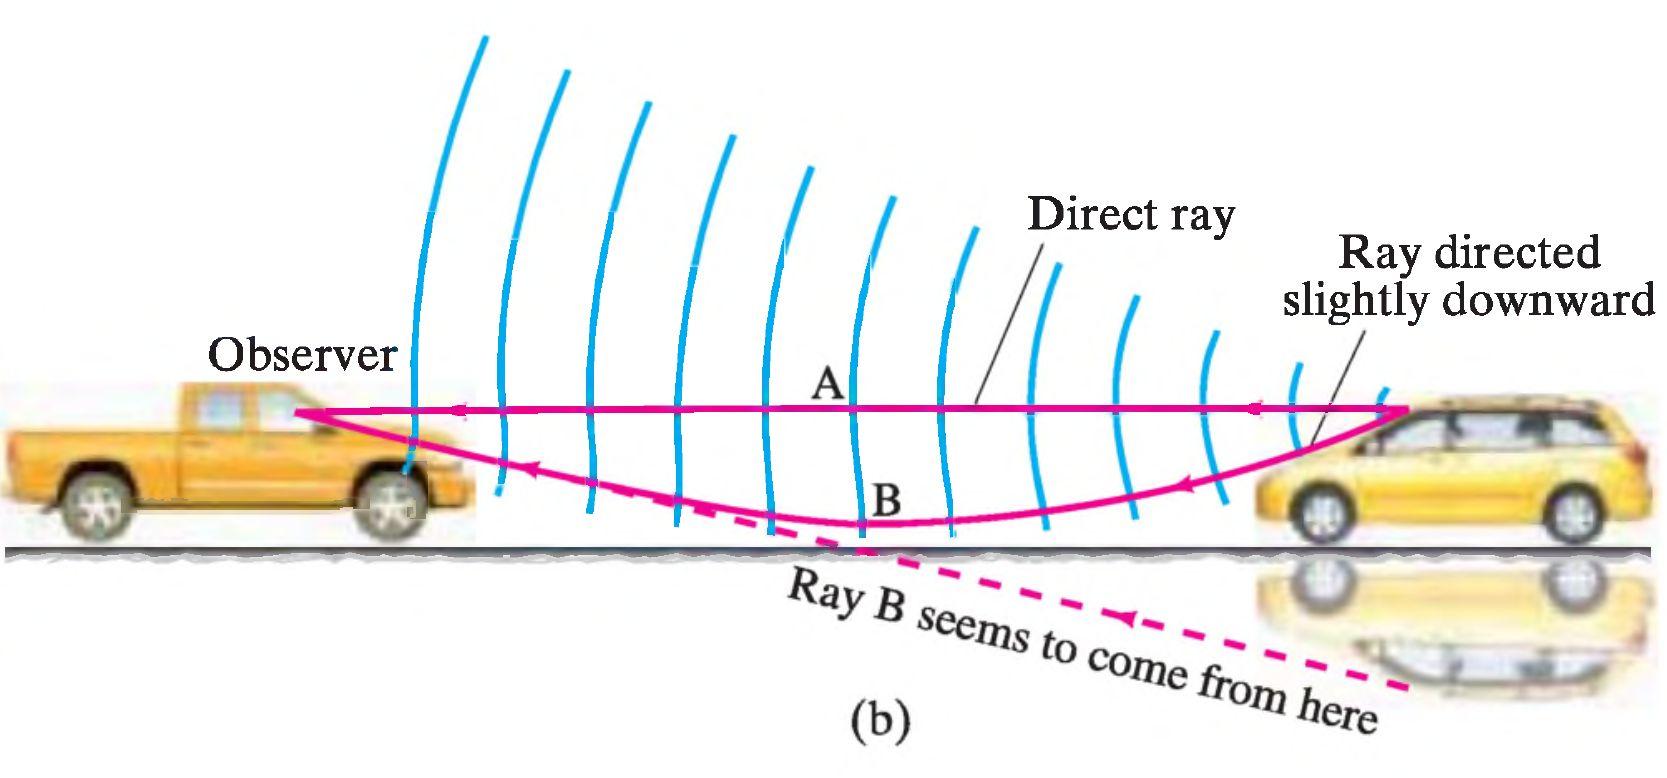
\includegraphics[height=1.7in]{images5/mirages.jpg}
\end{center}


  \end{frame}



%%%%%%%%%%%%%%%%%%%%%%%%%%%%%%%%%%%%%%%%%%%%%%%%%%%%%%%%%%%%%%%%%%%


\begin{frame}

\frametitle{Interference: Youn's double-slit Experiment}



\vspace{3mm}

  \begin{center}
  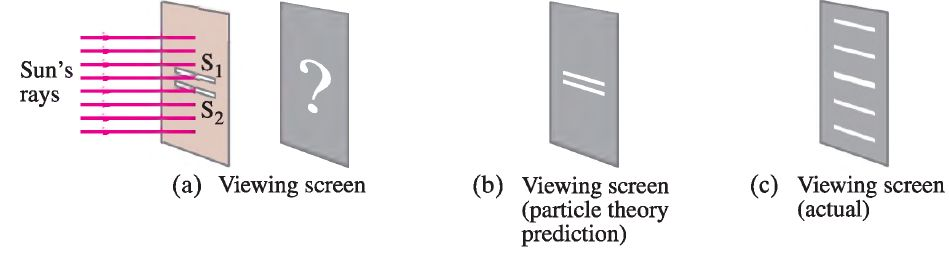
\includegraphics[height=1.2in]{images5/doubleslit.jpg}
\end{center}

\vspace{3mm}

If light consists of tiny particles, we might expect to see two bright lines on a screen placed behind
the slits as in (b). But instead a series of bright lines are seen, as in (c). Young was
able to explain this result as a wave-interference phenomenon.
  \end{frame}



%%%%%%%%%%%%%%%%%%%%%%%%%%%%%%%%%%%%%%%%%%%%%%%%%%%%%%%%%%%%%%%%%%%


\begin{frame}

\frametitle{Interference: Youn's double-slit Experiment}


To understand why, we consider:
\vspace{3mm}
\pause

\begin{itemize}
\item plane waves
\pause
\item single wavelength 
\end{itemize}

\pause

\vspace{3mm}

The waves leaving the two small slits spread out as shown:
\pause

\vspace{3mm}

  \begin{center}
  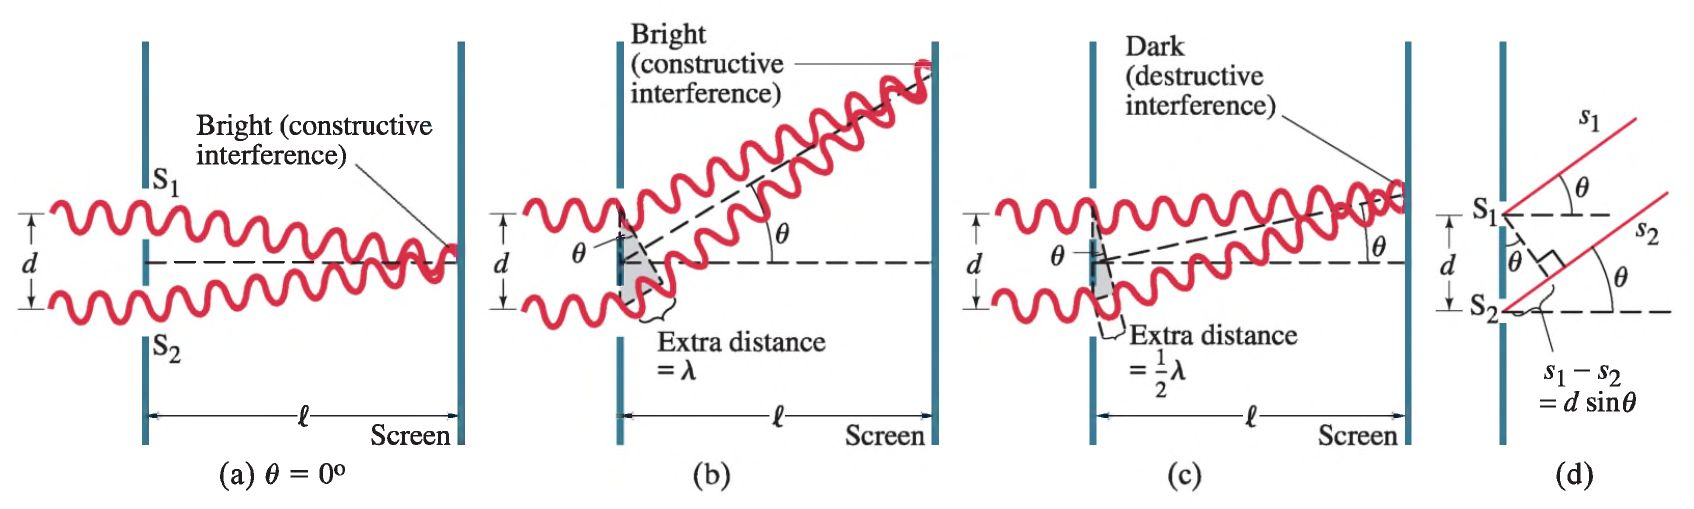
\includegraphics[height=1.2in]{images5/doubleslit2.jpg}
\end{center}


  \end{frame}




%%%%%%%%%%%%%%%%%%%%%%%%%%%%%%%%%%%%%%%%%%%%%%%%%%%%%%%%%%%%%%%%%%%


\begin{frame}

\frametitle{Interference: Youn's double-slit Experiment}

  \begin{center}
  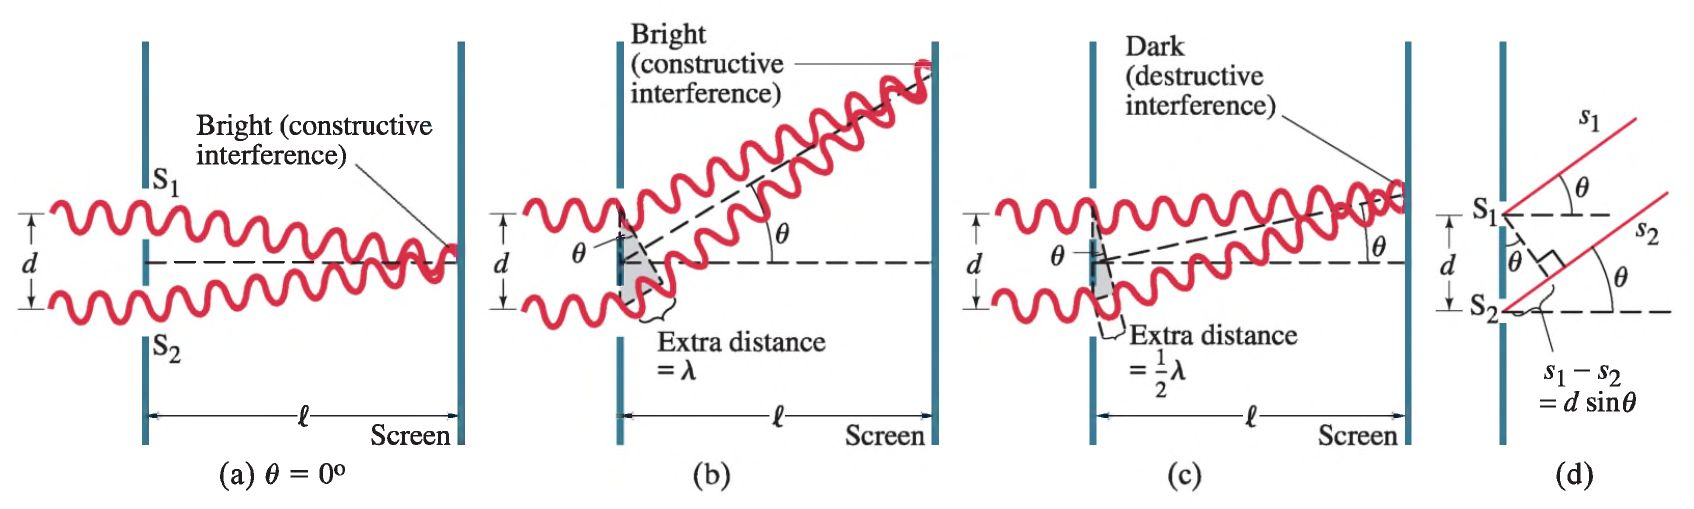
\includegraphics[height=1.2in]{images5/doubleslit2.jpg}
\end{center}

\pause


\begin{itemize}
\item Constructive interference $\rightarrow$ the path of 2 rays differs in $n \lambda$, $n$ integer.
\pause
\item Destructive interference $\rightarrow$ the path of 2 rays differs in  $(2n+1) \lambda/2$, $n$ integer.
\end{itemize}

\pause
\vspace{3mm}

Thus, there will be
a series of bright and dark lines (or fringes) on the viewing screen.

  \end{frame}



%%%%%%%%%%%%%%%%%%%%%%%%%%%%%%%%%%%%%%%%%%%%%%%%%%%%%%%%%%%%%%%%%%%


\begin{frame}

\frametitle{Interference: Youn's double-slit Experiment}

  \begin{center}
  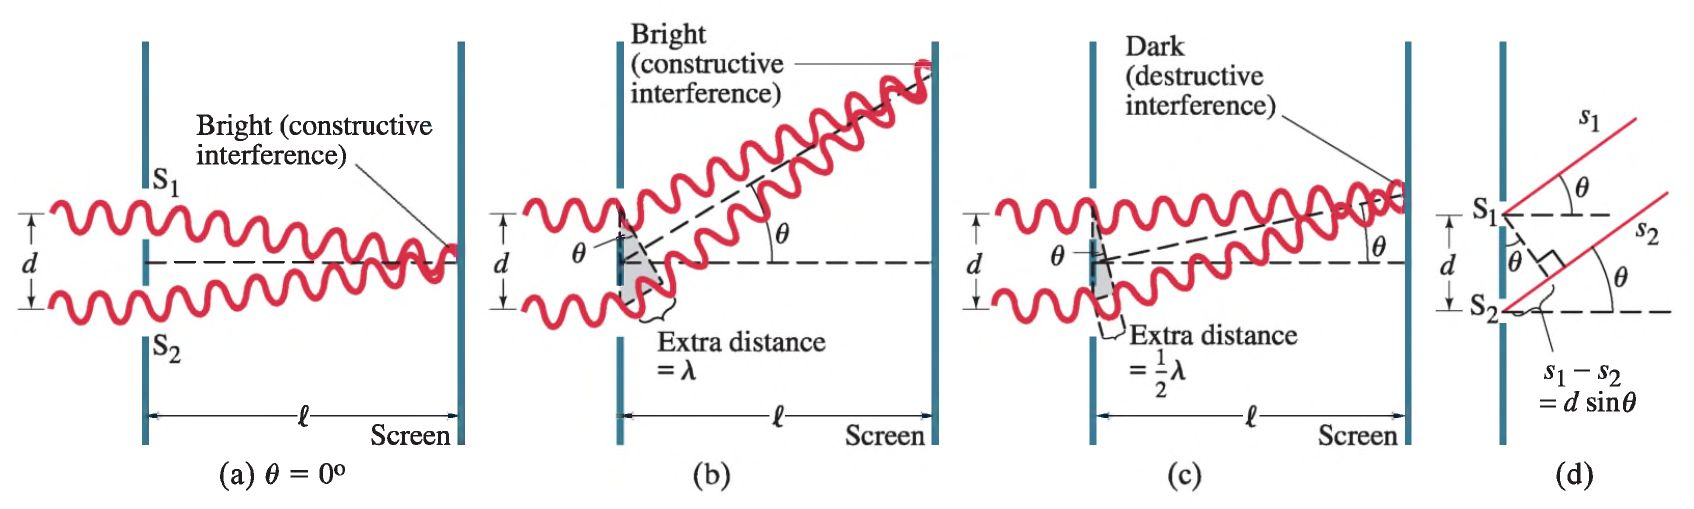
\includegraphics[height=1.2in]{images5/doubleslit2.jpg}
\end{center}

\pause
Where the bright lines fall?
\pause

\begin{itemize}
\item $d<<\ell$

\pause

\item The rays are essentially parallel.

\pause

\item $\theta$ is the angle they make with the horizontal.

\pause

\item The extra distance traveled by the lower ray is $d sin\theta$
\end{itemize}

  \end{frame}




%%%%%%%%%%%%%%%%%%%%%%%%%%%%%%%%%%%%%%%%%%%%%%%%%%%%%%%%%%%%%%%%%%%


\begin{frame}

\frametitle{Interference: Youn's double-slit Experiment}

  \begin{center}
  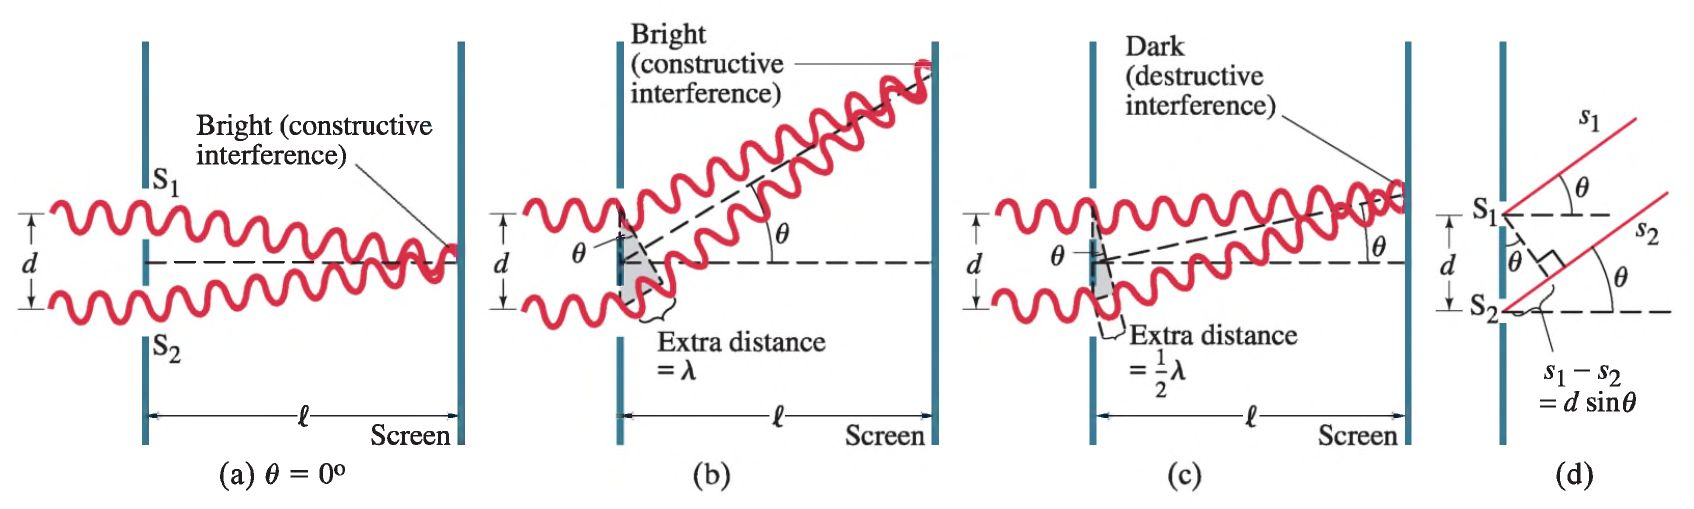
\includegraphics[height=1.2in]{images5/doubleslit2.jpg}
\end{center}

\pause
Where the bright lines fall?
\pause
\vspace{3mm}

Constructive interference:
\pause
\vspace{3mm}

\begin{equation}
 sin\theta=\frac{n\lambda}{d}=\frac{X}{\ell}
\end{equation}


  \end{frame}



%%%%%%%%%%%%%%%%%%%%%%%%%%%%%%%%%%%%%%%%%%%%%%%%%%%%%%%%%%%%%%%%%%%


\begin{frame}

\frametitle{Interference: Youn's double-slit Experiment}

  \begin{center}
  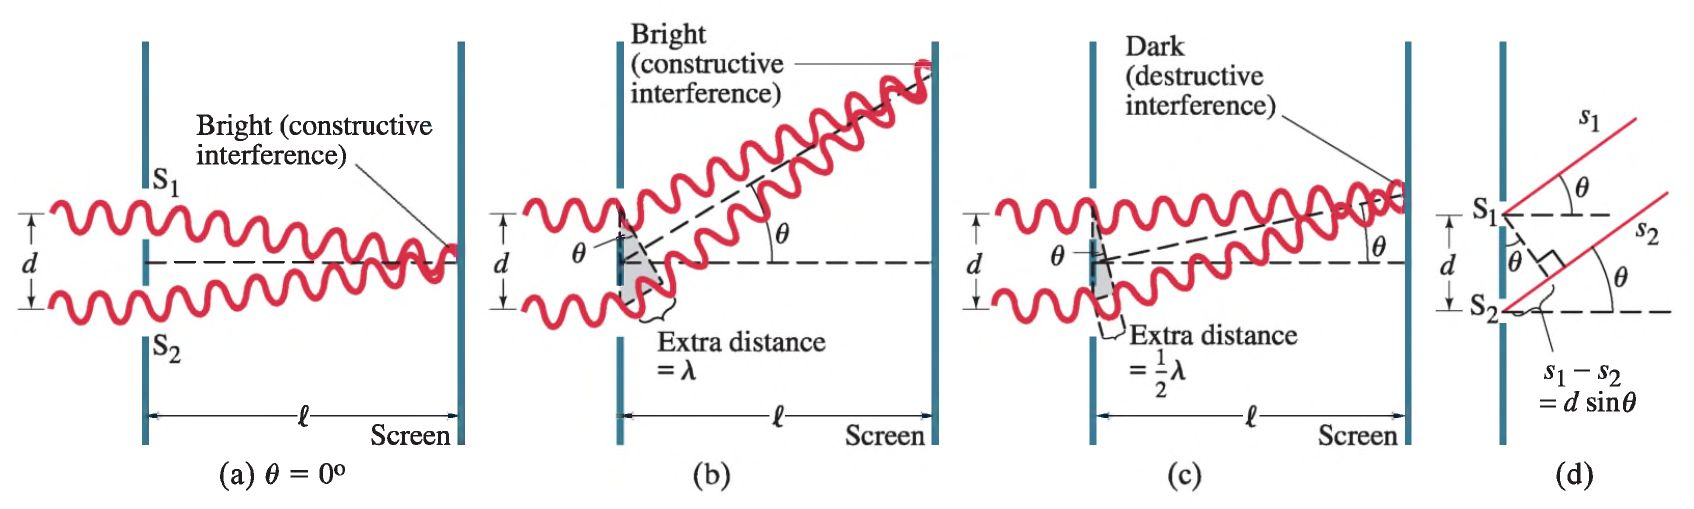
\includegraphics[height=1.2in]{images5/doubleslit2.jpg}
\end{center}


Where the bright lines fall?

\vspace{3mm}

Constructive interference:

\vspace{3mm}

\begin{equation}
 sin\theta=\frac{n\lambda}{d}=\frac{X}{\ell}\rightarrow X=\ell \frac{n\lambda}{d}
\end{equation}


  \end{frame}



%%%%%%%%%%%%%%%%%%%%%%%%%%%%%%%%%%%%%%%%%%%%%%%%%%%%%%%%%%%%%%%%%%%


\begin{frame}

\frametitle{Interference: Youn's double-slit Experiment}

  \begin{center}
  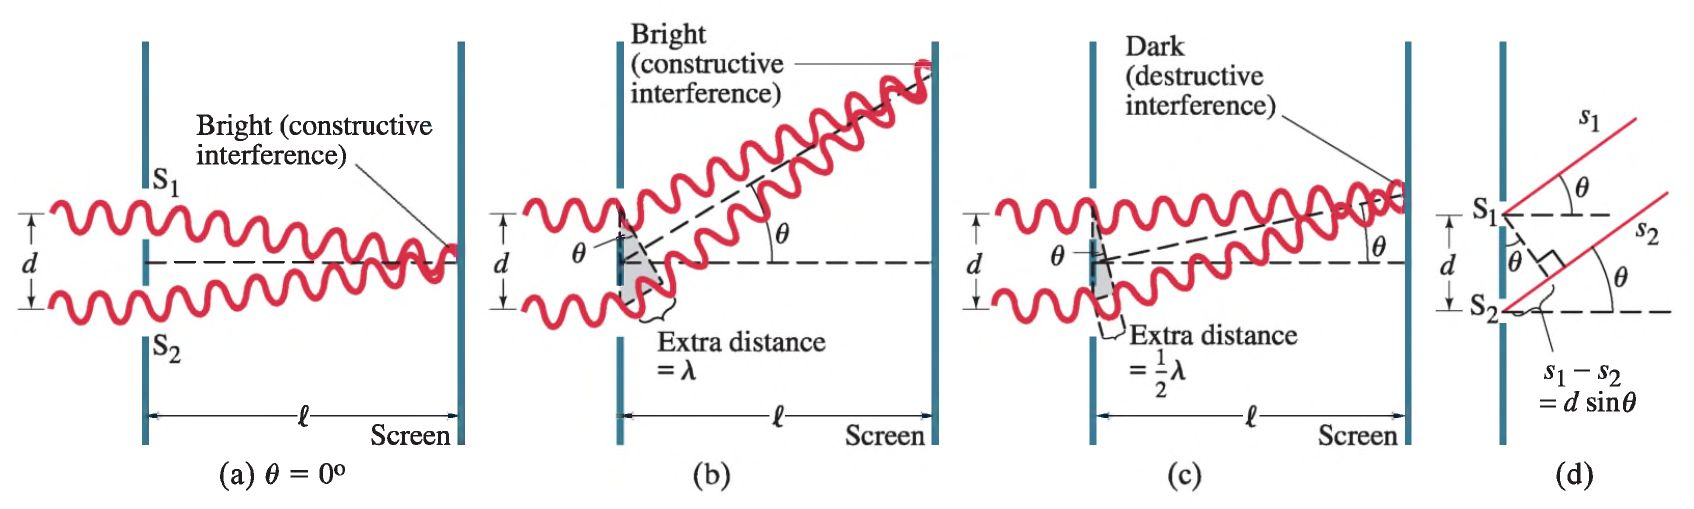
\includegraphics[height=1.2in]{images5/doubleslit2.jpg}
\end{center}


\pause


Destructive interference:
\pause
\vspace{3mm}

\begin{equation}
 sin\theta=\frac{(2n+1)\lambda}{d}=\frac{X}{\ell}
\end{equation}

  \end{frame}


%%%%%%%%%%%%%%%%%%%%%%%%%%%%%%%%%%%%%%%%%%%%%%%%%%%%%%%%%%%%%%%%%%%


\begin{frame}

\frametitle{Interference: Youn's double-slit Experiment}

  \begin{center}
  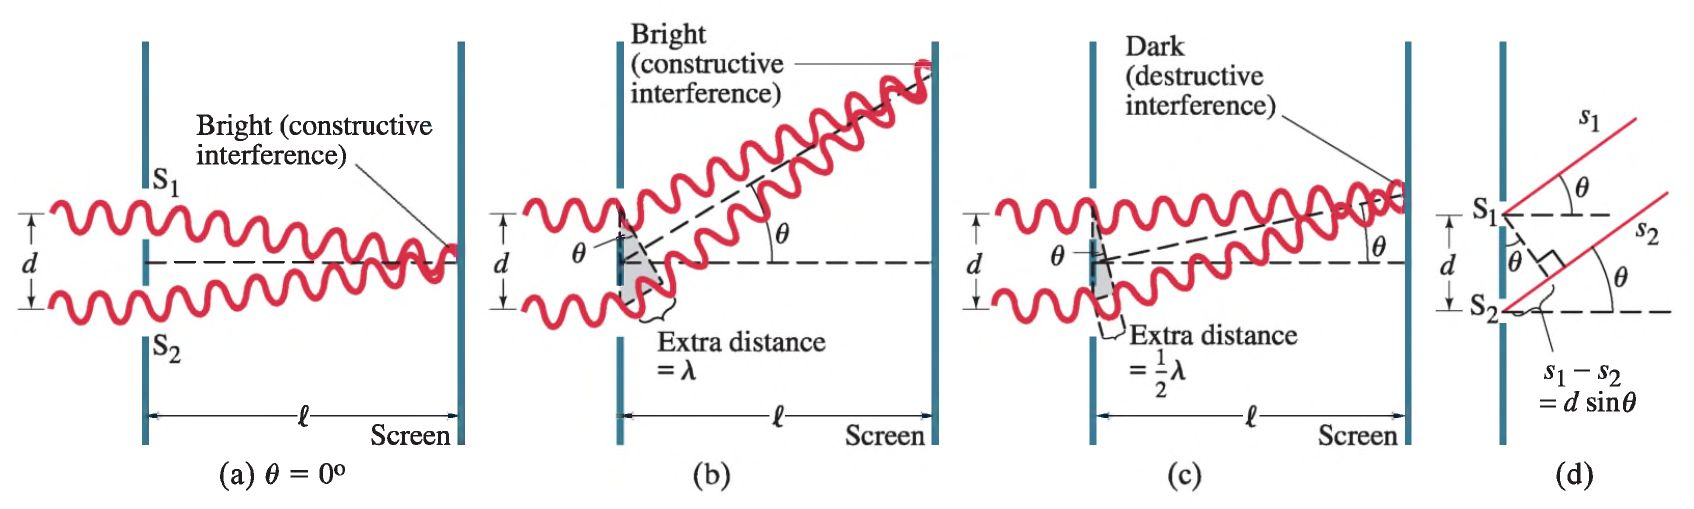
\includegraphics[height=1.2in]{images5/doubleslit2.jpg}
\end{center}


Where the bright lines fall?

\vspace{3mm}



Destructive interference:

\vspace{3mm}

\begin{equation}
 sin\theta=\frac{(2n+1)\lambda}{d}=\frac{X}{\ell}\rightarrow X=\ell \frac{(2n+1)\lambda}{d}
\end{equation}

  \end{frame}



%%%%%%%%%%%%%%%%%%%%%%%%%%%%%%%%%%%%%%%%%%%%%%%%%%%%%%%%%%%%%%%%%%%


\begin{frame}

\frametitle{Interference: Youn's double-slit Experiment}

Conceptual Example:
\vspace{3mm}

(a) Will there be an infinite number of points on the viewing screen where constructive and destructive
interference occur, or only a finite number of points? 
\vspace{3mm}
\pause

(b) Are neighboring points
of constructive interference uniformly spaced, or is the spacing between neighboring
points of constructive interference not uniform?

  \end{frame}


%%%%%%%%%%%%%%%%%%%%%%%%%%%%%%%%%%%%%%%%%%%%%%%%%%%%%%%%%%%%%%%%%%%


\begin{frame}

\frametitle{Interference: Youn's double-slit Experiment}

Conceptual Example:
\vspace{3mm}

(a) The maximum value of $n$ is the integer closest in value but smaller than d/X.
\vspace{3mm}
\pause

(b) For small values of $\theta$ the spacing is nearly uniform. For non-small values $\rightarrow$ the spacing gets larger as  $\theta$ gets larger.

  \end{frame}


%%%%%%%%%%%%%%%%%%%%%%%%%%%%%%%%%%%%%%%%%%%%%%%%%%%%%%%%%%%%%%%%%%%


\begin{frame}

\frametitle{Interference: Youn's double-slit Experiment}

Example:
\vspace{3mm}

A screen containing two slits $0.100~mm$ apart is $1.20~m$ from the viewing screen. Light of
wavelength $A = 500~nm$ falls on the slits from a distant source. Approximately
how far apart will adjacent bright interference fringes be on the screen?


  \begin{center}
  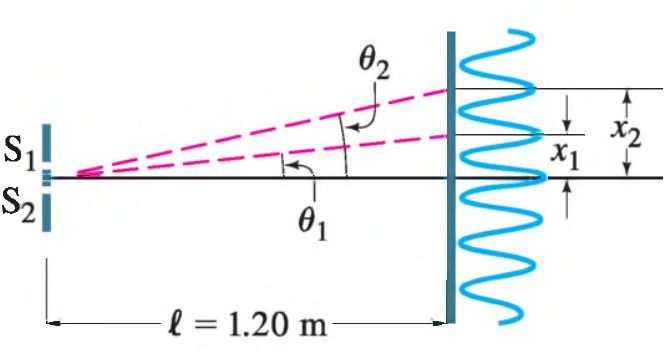
\includegraphics[height=1.2in]{images5/intexample.jpg}
\end{center}






  \end{frame}



%%%%%%%%%%%%%%%%%%%%%%%%%%%%%%%%%%%%%%%%%%%%%%%%%%%%%%%%%%%%%%%%%%%


\begin{frame}

\frametitle{Interference: Youn's double-slit Experiment}

Example:
\vspace{3mm}

  \begin{center}
  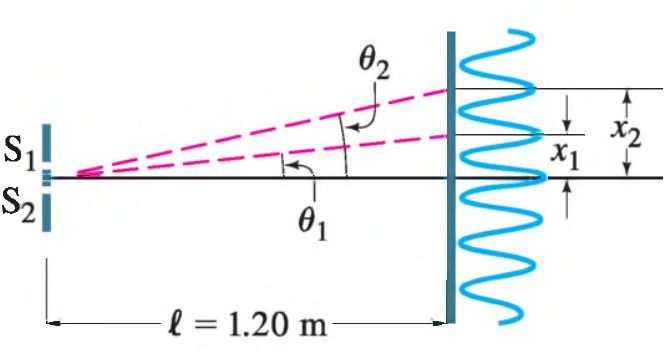
\includegraphics[height=1.2in]{images5/intexample.jpg}
\end{center}


\pause

\begin{equation}
sin\theta_1=\frac{m\lambda}{d}=\frac{(1)(500\times 10^{-9}~m)}{1.00\times 10^{-4}~m}=5.00\times 10^{-3}
\end{equation}


\pause
$\theta<<1\rightarrow sin\theta\sim \theta$ and $x_1/\ell =tan \theta_1\sim \theta_1$












  \end{frame}


%%%%%%%%%%%%%%%%%%%%%%%%%%%%%%%%%%%%%%%%%%%%%%%%%%%%%%%%%%%%%%%%%%%


\begin{frame}

\frametitle{Interference: Youn's double-slit Experiment}

Example:
\vspace{3mm}

then,



\begin{equation}
x_1\sim \ell \theta_1=(1.20~m)(5.00\times 10^{-3})=6.00~mm
\end{equation}
\pause


\begin{equation}
x_2\sim \ell \theta_2=\ell \frac{2\lambda}{d}=12.00~mm
\end{equation}
\pause

Thus the lower order fringes are 6.00 mm apart.






  \end{frame}
%%%%%%%%%%%%%%%%%%%%%%%%%%%%%%%%%%%%%%%%%%%%%%%%%%%%%%%%%%%%%%%%%%%


\begin{frame}

\frametitle{Interference: Youn's double-slit Experiment}

Conceptual Example:
\vspace{3mm}

(a) What happens to the interference pattern, if the incident light
(500 nm) is replaced by light of wavelength 700 nm? (b) What happens instead if the
wavelength stays at 500 nm but the slits are moved farther apart?

  \end{frame}




%%%%%%%%%%%%%%%%%%%%%%%%%%%%%%%%%%%%%%%%%%%%%%%%%%%%%%%%%%%%%%%%%%%


\begin{frame}

\frametitle{Interference: Youn's double-slit Experiment}
Except for the zeroth-order fringe at the center, the position of the fringes depends on wavelength.

\vspace{3mm}

  \begin{center}
  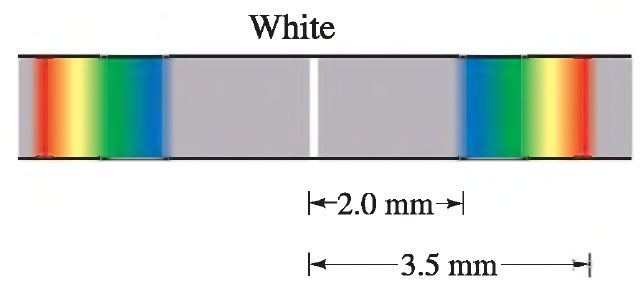
\includegraphics[height=1.2in]{images5/colors.jpg}
\end{center}

  \end{frame}


%%%%%%%%%%%%%%%%%%%%%%%%%%%%%%%%%%%%%%%%%%%%%%%%%%%%%%%%%%%%%%%%%%%


%\begin{frame}

%\frametitle{Coerence}



%\begin{itemize}
%\item Coherent sources $\rightarrow$ the waves have the same wavelength and frequency, 
%and bear the same phase relationship to each other at all times. 
%\pause 

%\item Incoherent sources $\rightarrow$ waves have phases that bear no fixed relationship to each other 
%over time
%\end{itemize}

%\pause

 %An interference pattern is observed
%only when the sources are coherent. If two tiny lightbulbs replaced the two slits, an
%interference pattern would not be seen. The light emitted by one lightbulb would
%have a random phase with respect to the second bulb, and the screen would be
%more or less uniformly illuminated. 

%  \end{frame}


%%%%%%%%%%%%%%%%%%%%%%%%%%%%%%%%%%%%%%%%%%%%%%%%%%%%%%%%%%%%%%%%%%%


\begin{frame}

\frametitle{Intensity in the Interference Pattern}



\begin{itemize}

\item $E_{\theta}=E_1+E_2$
\pause

\item $E_1=E_{10}sin\omega t$
\pause

\item $E_2=E_{20}sin(\omega t+\delta)$, $\frac{\delta}{2\pi}=\frac{dsin\theta}{\lambda}$


\end{itemize}

We can work with this expression and prove that:

\begin{equation}
\frac{I_{\theta}}{I_0}=\frac{E^2_{\theta 0}}{(2E_0)^2}=cos^2\frac{\delta}{2}
\end{equation}

  \end{frame}
  
  
  

%%%%%%%%%%%%%%%%%%%%%%%%%%%%%%%%%%%%%%%%%%%%%%%%%%%%%%%%%%%%%%%%%%%


\begin{frame}

\frametitle{Intensity in the Interference Pattern}






\begin{equation}
I_{\theta}=I_0cos^2\left(\frac{\pi d sin \theta}{\lambda}\right)
\end{equation}

\pause
small $\theta$, $sin\theta=\frac{y}{\ell}$


\begin{equation}
I_{\theta}=I_0\left[cos\left(\frac{\pi d }{\lambda \ell} y\right)\right]^2
\end{equation}


  \end{frame}





%%%%%%%%%%%%%%%%%%%%%%%%%%%%%%%%%%%%%%%%%%%%%%%%%%%%%%%%%%%%%%%%%%%


\begin{frame}

\frametitle{Intensity in the Interference Pattern}

  \begin{center}
  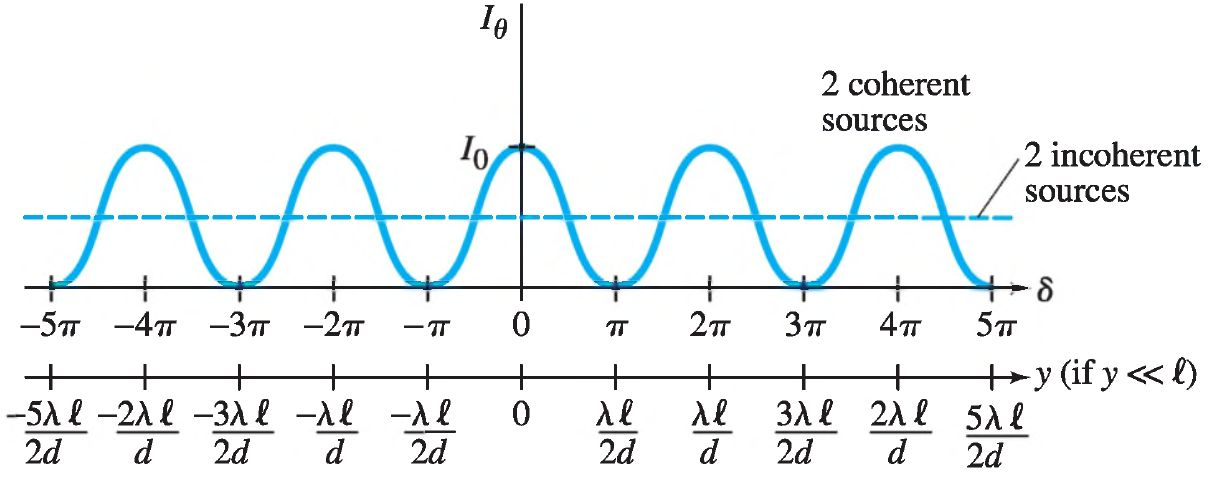
\includegraphics[height=1.5in]{images5/intensity.jpg}
\end{center}

\pause

The intensity pattern shows a series of maxima of equal height, and is based on the assumption that
each slit (alone) would illuminate the screen uniformly. This is never quite true, if we consider  diffraction. 



  \end{frame}




%%%%%%%%%%%%%%%%%%%%%%%%%%%%%%%%%%%%%%%%%%%%%%%%%%%%%%%%%%%%%%%%%%%


\begin{frame}

\frametitle{Interference in Thin Films}

  \begin{center}
  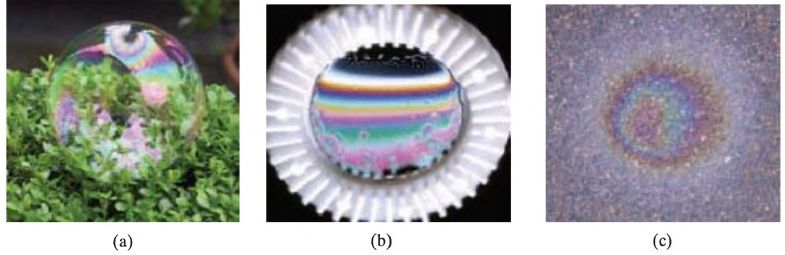
\includegraphics[height=1.7in]{images5/soap.jpg}
\end{center}


  \end{frame}


%%%%%%%%%%%%%%%%%%%%%%%%%%%%%%%%%%%%%%%%%%%%%%%%%%%%%%%%%%%%%%%%%%%


\begin{frame}

\frametitle{Interference in Thin Films}




  \begin{columns}[c]
   \column{2in}  % slides are 3in high by 5in wide
  
    \begin{center}
  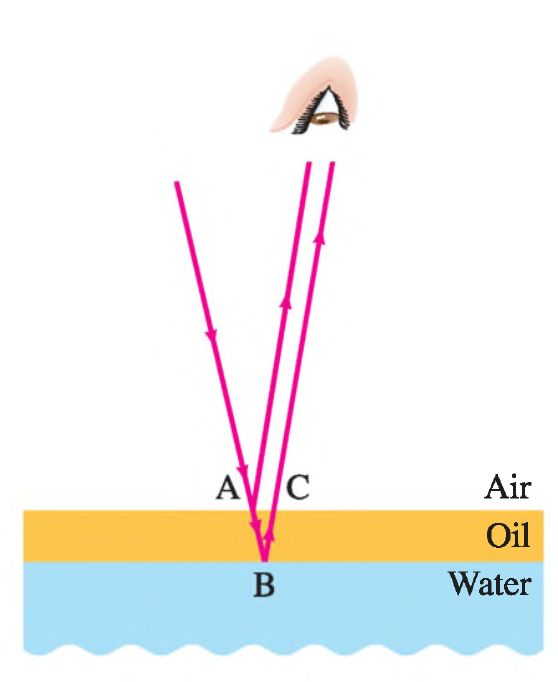
\includegraphics[height=1.7in]{images5/soap2.jpg}
\end{center}
  
  
   \column{2in}


If path difference $ABC$ is,

\begin{itemize}
\item equals $m\lambda_n\rightarrow$ constructive interference
\pause
\item equals $(2m+1)\lambda_n\rightarrow$ destructive interference
\pause
\item $\lambda_n=\lambda/n$, $n$ is the index of refraction
\end{itemize}


   \end{columns}


  \end{frame}


%%%%%%%%%%%%%%%%%%%%%%%%%%%%%%%%%%%%%%%%%%%%%%%%%%%%%%%%%%%%%%%%%%%


\begin{frame}

\frametitle{Newton's Rings}


   \begin{center}
  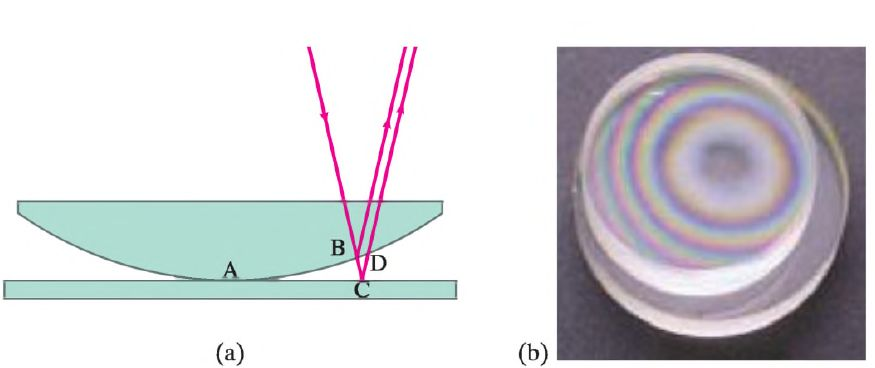
\includegraphics[height=1.7in]{images5/rings.jpg}
\end{center}
  



  \end{frame}



%%%%%%%%%%%%%%%%%%%%%%%%%%%%%%%%%%%%%%%%%%%%%%%%%%%%%%%%%%%%%%%%%%%


\begin{frame}

\frametitle{Newton's Rings}


 Why is the center dark?
 

   \begin{columns}[c]
   \column{2in}  % slides are 3in high by 5in wide
  
\pause

   \begin{center}
  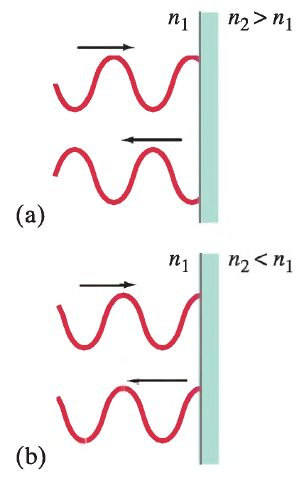
\includegraphics[height=1.7in]{images5/reflexion.jpg}
\end{center}

   \column{2in}


\textbf{a beam of light reflected by a material with index of refraction greater than
that of the material in which it is traveling, changes phase by 180° or $\frac{1}{2}$ cycle;}



   \end{columns}

 



  \end{frame}




%%%%%%%%%%%%%%%%%%%%%%%%%%%%%%%%%%%%%%%%%%%%%%%%%%%%%%%%%%%%%%%%%%%


\begin{frame}

\frametitle{Colors in a Thin Soap Film}




  \begin{columns}[c]
   \column{2in}  % slides are 3in high by 5in wide
  
  
     \begin{center}
  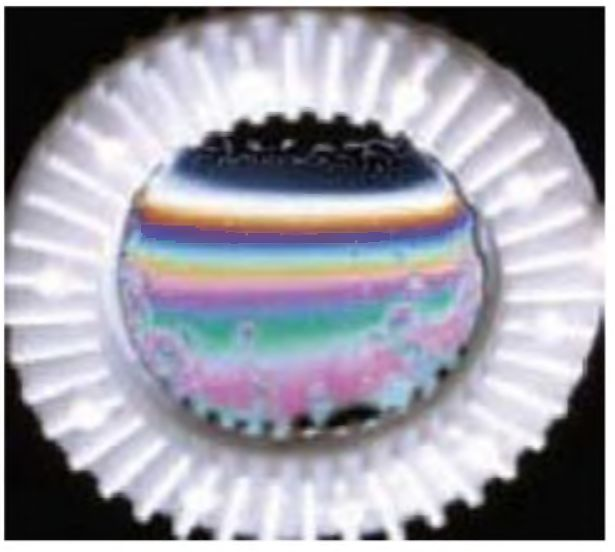
\includegraphics[height=1.7in]{images5/soap3.jpg}
\end{center}


   \column{2in}

  
  \begin{itemize}
  \item The thin film  stood vertically.
  \pause
 \item  Gravity has pulled much of the soapy water toward the bottom.
 
 \pause
\item The top section is so thin $\rightarrow$ light reflected from the front and
back surfaces have almost no path difference.

\pause

\item 180$^{\circ}$ $\rightarrow$  two reflected waves are  out of phase for all wavelengths.

 
  
  \end{itemize}
  


   \end{columns}




  \end{frame}



%%%%%%%%%%%%%%%%%%%%%%%%%%%%%%%%%%%%%%%%%%%%%%%%%%%%%%%%%%%%%%%%%%%


\begin{frame}

\frametitle{Colors in a Thin Soap Film}


  
     \begin{center}
  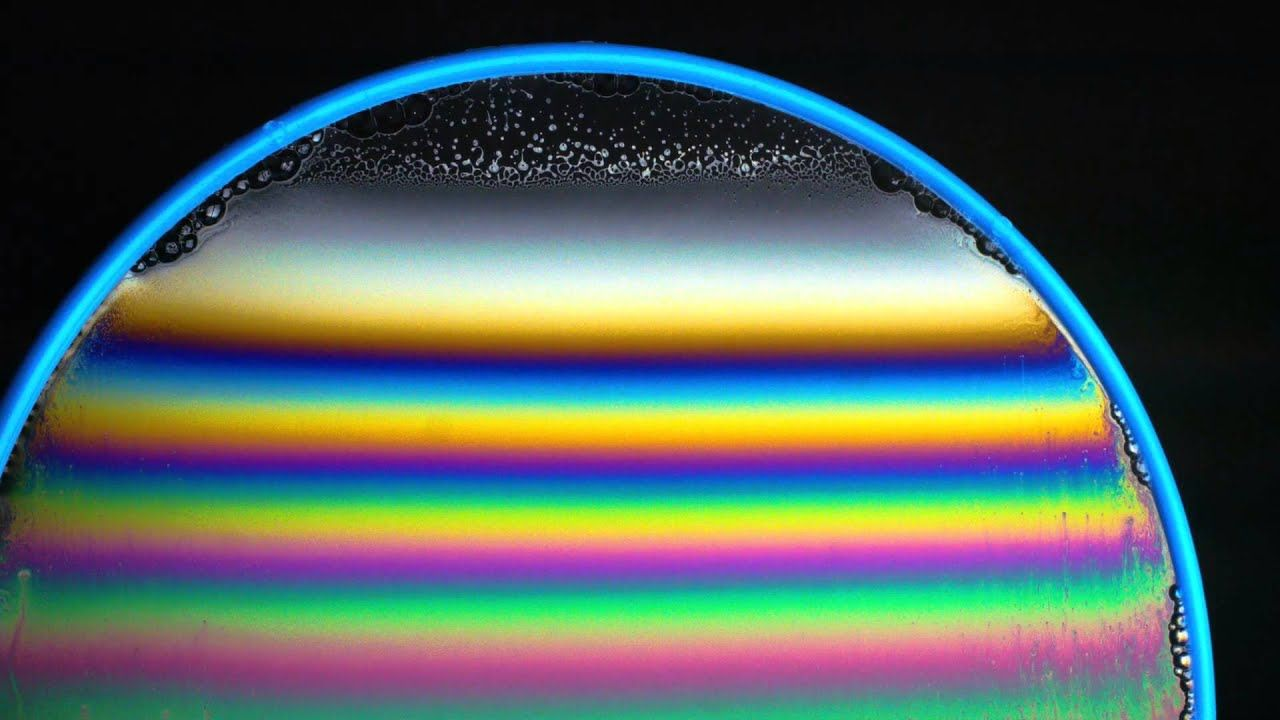
\includegraphics[height=2.0in]{images5/soap4.jpg}
\end{center}



  \end{frame}

%%%%%%%%%%%%%%%%%%%%%%%%%%%%%%%%%%%%%%%%%%%%%%%%%%%%%%%%%%%%%%%%%%%


\begin{frame}

\frametitle{Colors in a Thin Soap Film}


  
     \begin{center}
  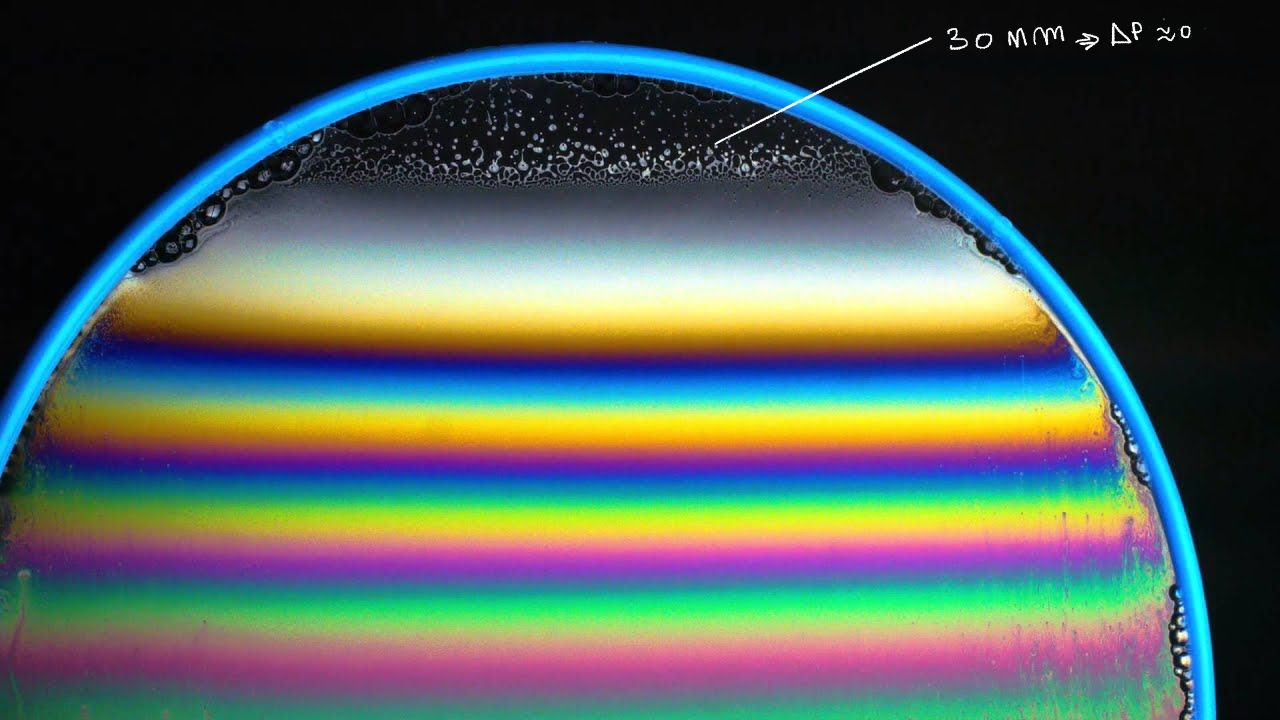
\includegraphics[height=2.0in]{images5/soap4b.jpg}
\end{center}



  \end{frame}



%%%%%%%%%%%%%%%%%%%%%%%%%%%%%%%%%%%%%%%%%%%%%%%%%%%%%%%%%%%%%%%%%%%


\begin{frame}

\frametitle{Colors in a Thin Soap Film}


  
     \begin{center}
  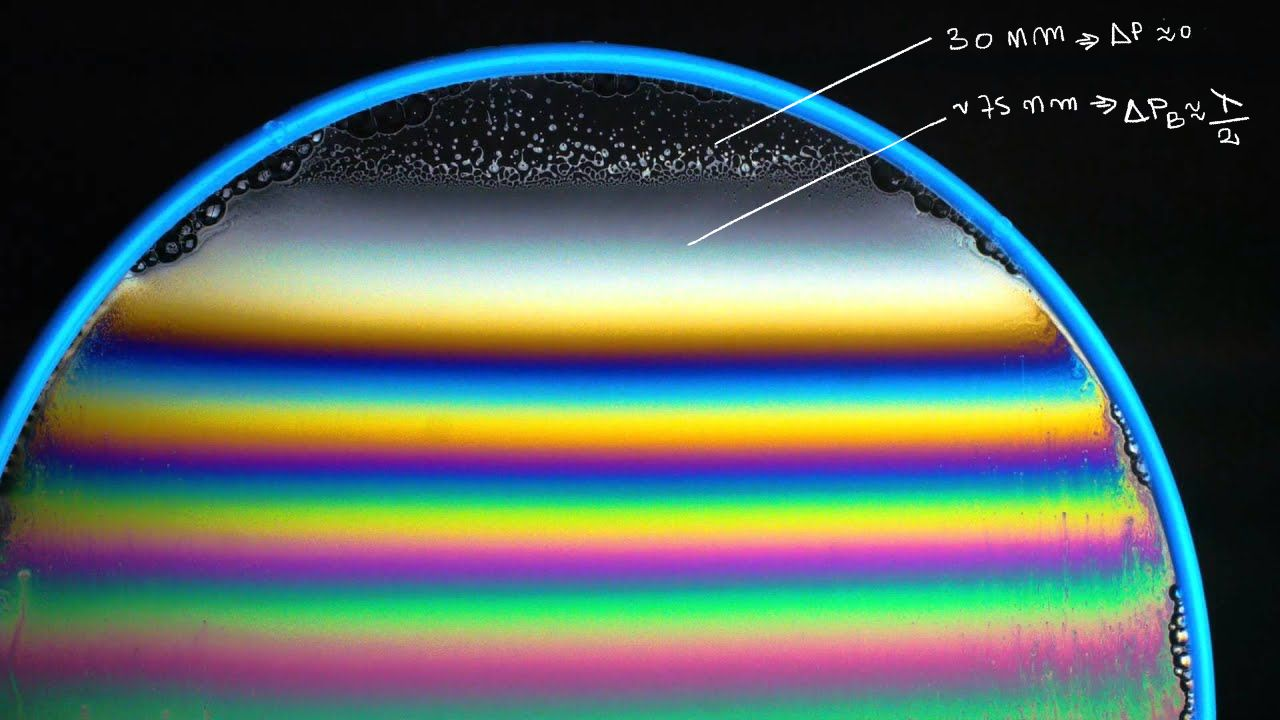
\includegraphics[height=2.0in]{images5/soap4c.jpg}
\end{center}



  \end{frame}



%%%%%%%%%%%%%%%%%%%%%%%%%%%%%%%%%%%%%%%%%%%%%%%%%%%%%%%%%%%%%%%%%%%


\begin{frame}

\frametitle{Colors in a Thin Soap Film}


  
     \begin{center}
  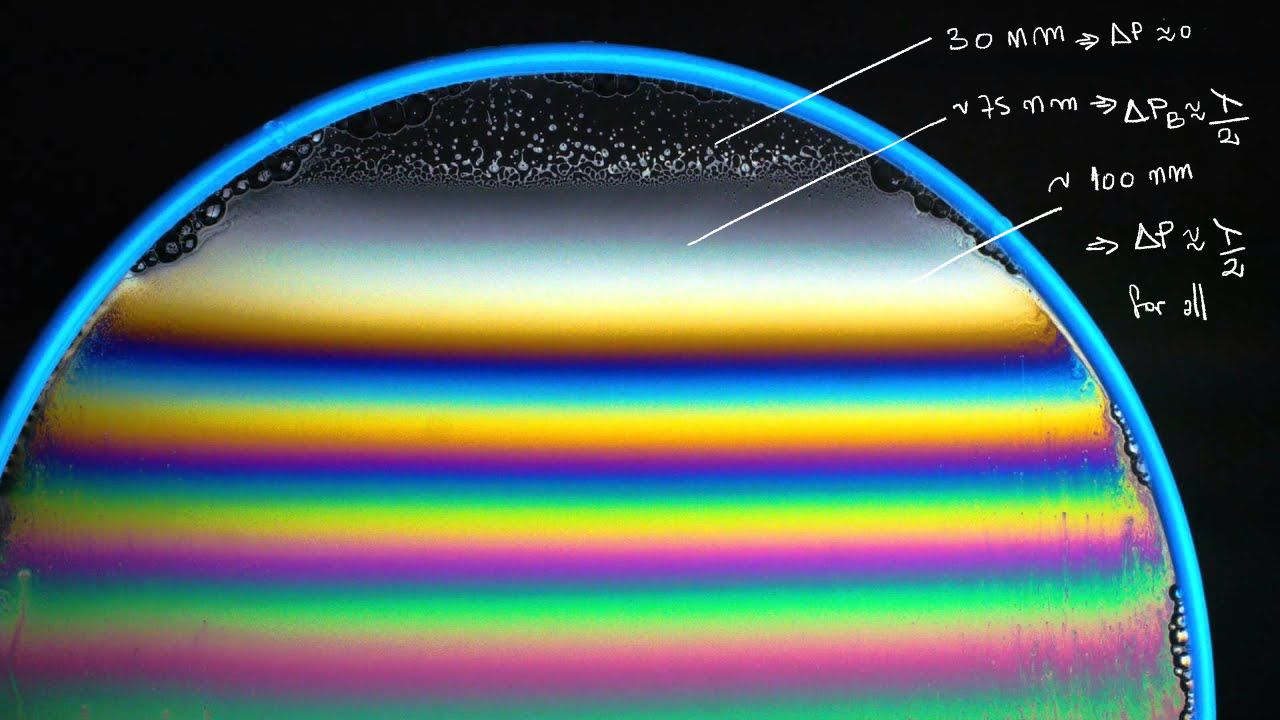
\includegraphics[height=2.0in]{images5/soap4d.jpg}
\end{center}



  \end{frame}

%%%%%%%%%%%%%%%%%%%%%%%%%%%%%%%%%%%%%%%%%%%%%%%%%%%%%%%%%%%%%%%%%%%


\begin{frame}

\frametitle{Colors in a Thin Soap Film}


  
     \begin{center}
  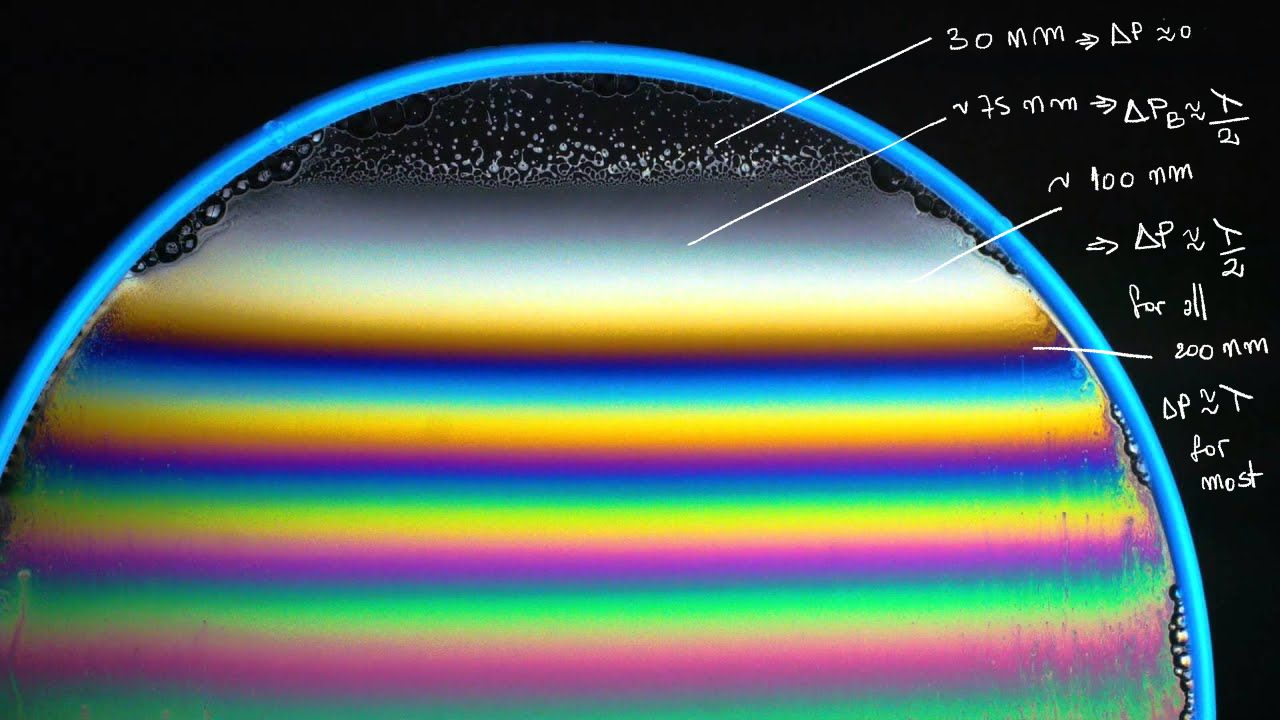
\includegraphics[height=2.0in]{images5/soap4e.jpg}
\end{center}



  \end{frame}

%%%%%%%%%%%%%%%%%%%%%%%%%%%%%%%%%%%%%%%%%%%%%%%%%%%%%%%%%%%%%%%%%%%


\begin{frame}

\frametitle{Colors in a Thin Soap Film}


  
     \begin{center}
  \includegraphics[height=2.0in]{images5/soap4f.jpg}
\end{center}



  \end{frame}


%%%%%%%%%%%%%%%%%%%%%%%%%%%%%%%%%%%%%%%%%%%%%%%%%%%%%%%%%%%%%%%%%%%


\begin{frame}

\frametitle{Michelson Interferometer}



    \begin{center}
  \includegraphics[height=1.9in]{images5/Michelson2.jpg}
\end{center}



  \end{frame}









%%%%%%%%%%%%%%%%%%%%%%%%%%%%%%%%%%%%%%%%%%%%%%%%%%%%%%%%%%%%%%%%%%%


\begin{frame}

\frametitle{Questions}


\begin{itemize}
\item Does Huygens’ principle apply to sound waves? To water
waves?
\pause

\item We can hear sounds around corners but we cannot see
around corners; yet both sound and light are waves. Explain
the difference.
\pause

\item  Two rays of light from the same source destructively interfere
if their path lengths differ by how much?







\end{itemize}


  \end{frame}











%%%%%%%%%%%%%%%%%%%%%%%%%%%%%%%%%%%%%%%%%%%%%%%%%%%%%%%%%%%%%%%%%%%


\begin{frame}

\frametitle{Questions}


\begin{itemize}

\item Monochromatic red light is incident on a double slit and the
interference pattern is viewed on a screen some distance
away. Explain how the fringe pattern would change if the
red light source is replaced by a blue light source.

\pause

\item Compare a double-slit experiment for sound waves to that
for light waves. Discuss the similarities and differences.


\end{itemize}


  \end{frame}





























%%%%%%%%%%%%%%%%%%%%%%%%%%%%%%%%%%%%%%%%%%%%%%%%%%%%%%%%%%%%%%%
 \end{document}
%%%%%%%%%%%%%%%%%%%%%%%%%%%%%%%%%%%%%%%%%%%%%%%%%%%%%%%%%%%%%%%